% ============================================================================
%  Radicle Beyond the One Big Room -- An Economic and Architectural Case
%  Standalone critique and proposal. Assumes the context of the Sovereign Bunny
%  whitebooklet (sovereign-booklet.tex) and may cite it, but depends on no
%  Sovereign Bunny component: a ledger is optional throughout.
%  Build:   make -C docs/booklet radicle-pdf   (run on the remote build host only)
% ============================================================================
\documentclass[a4paper,11pt,twoside,parskip=half-,headings=small]{scrartcl}

% ============================================================================
%  common-preamble.tex -- shared packages, colours, boxes and status macros for
%  the Sovereign Bunny paper set (all papers except the base booklet, which
%  keeps its own preamble). Each paper sets its own \documentclass, hyperref
%  metadata and fancyhdr heads (see \setpaperheads).
% ============================================================================
\usepackage[T1]{fontenc}
\usepackage[utf8]{inputenc}
\usepackage{lmodern}
\usepackage[english]{babel}
\usepackage{microtype}
\setlength{\emergencystretch}{2em}
\usepackage[margin=2.5cm,headheight=14pt]{geometry}
\usepackage{amsmath,amssymb}
\usepackage{booktabs,tabularx,longtable,array}
\usepackage{xcolor}
\usepackage{tikz}
\usetikzlibrary{arrows.meta,positioning,shapes.geometric,fit,calc,backgrounds}
\usepackage{caption}
\usepackage{needspace}
\usepackage{enumitem}
\usepackage{tcolorbox}
\tcbuselibrary{breakable}
\usepackage{listings}
\usepackage{fancyhdr}
\usepackage{float}
\usepackage{ragged2e}
\usepackage[hidelinks]{hyperref}
\usepackage[capitalise,noabbrev]{cleveref}

\setlength{\parindent}{0pt}
\captionsetup{font=small,labelfont=bf,justification=centering}

\definecolor{ink}{HTML}{1B2A41}
\definecolor{accent}{HTML}{0B7A75}
\definecolor{warn}{HTML}{B5472B}
\definecolor{mute}{HTML}{5C6B7A}
\definecolor{codebg}{HTML}{F8FAFC}
\addtokomafont{section}{\color{ink}}
\addtokomafont{subsection}{\color{ink}}
\addtokomafont{subsubsection}{\color{ink}}
\setlist{itemsep=2pt,topsep=4pt}

\lstdefinestyle{customcode}{
  backgroundcolor=\color{codebg},commentstyle=\color{mute}\itshape,
  keywordstyle=\color{accent}\bfseries,stringstyle=\color{warn},
  basicstyle=\ttfamily\scriptsize,breaklines=true,captionpos=b,keepspaces=true,
  showstringspaces=false,frame=single,rulecolor=\color{mute!30},tabsize=2}
\lstdefinelanguage{Rust}{
  keywords={true,false,struct,enum,fn,let,mut,pub,impl,for,if,else,match,return,const,u8,u16,u32,u64,usize,bool,String,Vec,Result,Ok,Err,Option,Some,None,use,self,Self},
  sensitive=true,comment=[l]{//},morecomment=[s]{/*}{*/},morestring=[b]"}
\lstdefinelanguage{JSON}{
  string=[s]{"}{"},stringstyle=\color{warn},comment=[l]{//},
  morekeywords={true,false,null},keywordstyle=\color{accent}\bfseries}
\lstdefinelanguage{TypeScript}{
  keywords={export,interface,type,const,let,function,async,await,return,import,from,new,readonly,number,string,bigint,boolean,void,Promise,Map,Uint8Array,ReadableStream,true,false},
  sensitive=true,comment=[l]{//},morecomment=[s]{/*}{*/},morestring=[b]",morestring=[b]'}
\lstset{style=customcode}

\pagestyle{fancy}
\fancyhf{}
\fancyfoot[C]{\small\thepage}
\renewcommand{\headrulewidth}{0.3pt}

\IfFileExists{build/meta.tex}{\input{build/meta.tex}}{%
  \newcommand{\bookletcommit}{unversioned}%
  \newcommand{\bookletdate}{\today}}

\newcommand{\EUR}[1]{\texteuro\,#1}
\newcommand{\code}[1]{\texttt{#1}}
\newcommand{\claim}[1]{\textcolor{warn}{[#1]}}
\newcommand{\stImpl}{\textcolor{accent}{\textbf{Implemented}}}
\newcommand{\stPart}{\textcolor{mute}{\textbf{Partial}}}
\newcommand{\stStub}{\textcolor{warn}{\textbf{Stub / unsafe}}}
\newcommand{\stSpec}{\textcolor{mute}{\textbf{Specified}}}
\newcommand{\stPlan}{\textcolor{mute}{\textbf{Planned}}}
\newcommand{\stRes}{\textcolor{warn}{\textbf{Research}}}
\newcolumntype{L}[1]{>{\RaggedRight\arraybackslash}p{#1}}
\newcolumntype{Y}{>{\RaggedRight\arraybackslash}X}

\newtcolorbox{keybox}[2][]{%
  breakable,colback=accent!6,colframe=accent,boxrule=0.6pt,arc=2pt,
  left=7pt,right=7pt,top=3pt,bottom=3pt,
  fonttitle=\bfseries,coltitle=accent,colbacktitle=accent!6,
  title={#2},before skip=4pt,after skip=4pt,#1}
\newtcolorbox{warnbox}[2][]{%
  breakable,colback=warn!5,colframe=warn,boxrule=0.6pt,arc=2pt,
  left=7pt,right=7pt,top=4pt,bottom=4pt,
  fonttitle=\bfseries,coltitle=warn,colbacktitle=warn!5,
  title={#2},before skip=6pt,after skip=6pt,#1}

\raggedbottom
\newcommand{\setpaperheads}[2]{\fancyhead[LE,RO]{\small\color{mute}#1}\fancyhead[RE,LO]{\small\color{mute}#2}}
\newcommand{\booklet}{the Sovereign Bunny whitebooklet}

\hypersetup{pdftitle={Radicle Beyond the One Big Room: An Economic and Architectural Case},pdfauthor={Sovereign Bunny contributors},pdfsubject={Network-scoped identity, polycentric meshes, and a sustainable economic model for sovereign code collaboration},pdfkeywords={radicle, did:rad, iroh, polycentric, mesh, sovereignty}}
\setpaperheads{Radicle Beyond the One Big Room}{Sovereign Bunny paper set -- Radicle}

\begin{document}

% ============================================================================
\begin{titlepage}
  \centering
  \vspace*{2.2cm}
  {\color{mute}\scshape\large Paper \& Architectural Proposal\par}
  \vspace{0.6cm}
  {\color{ink}\Huge\bfseries Radicle Beyond the One Big Room\par}\vspace{0.4cm}
  {\color{accent}\Large An Economic Case and a Technical Remedy for\\Monolithic Network Assumptions in Sovereign Code Collaboration\par}
  \vspace{0.8cm}
  {\large Network-scoped identity, polycentric meshes, and a funding model that survives disagreement\par}
  \vfill
  \begin{tabular}{rl}
    \textbf{Status}   & Draft -- standalone; assumes whitebooklet v0.5 context\\
    \textbf{Revision} & \code{\bookletcommit}\\
    \textbf{Built}    & \bookletdate\\
    \textbf{Licence}  & CC BY-SA 4.0 (text); Apache-2.0 (code samples)\\
  \end{tabular}
  \vspace{1.0cm}

  \begin{minipage}{0.84\textwidth}\small\color{mute}
  Claims about third-party software carry one of three tags. \claim{verified} means we checked a primary source on 2026-10-17 (the project's FAQ and security disclosure page, the Radicle Garden service page, or the cited paper). \claim{reported} means a source-level claim (code, configuration, version numbers) supplied by a reviewer that we have not independently re-checked. \claim{unverified} marks working hypotheses. All tags are collected in \cref{sec:verify}. Nothing here is a criticism of the people maintaining
  Radicle: it is an invitation to finish a job whose hardest half they already did.
  \end{minipage}
  \vspace*{1.2cm}
\end{titlepage}

\begin{abstract}
\noindent
Radicle freed source-code collaboration from a single global execution state
machine. Repositories are fragmented Git namespaces, peers track only what they
choose to track, and issues and patches merge asynchronously as collaborative
objects. At the data layer it is already pluralist. At the network layer, however,
it still inherits a mental model from the chains it escaped: one ambient peer pool,
a handful of load-bearing public seeds, and an identity namespace that is blind to
the trust perimeter it operates in.

\noindent
This paper makes two arguments. First, an \emph{economic} one: a protocol whose
maintainers carry a global commons on volunteer willpower will burn out, and the
fix is not more grants but a deliberate split between a free, uncapturable core and
paid, SLA-backed services around it, in the manner of Linux and its distribution
ecosystem. The decisive design property is that anyone can run their own network,
including people who disagree with the maintainers. Second, a \emph{technical} one:
we propose network-scoped identifiers (\code{did:rad:<network\_id>:<subject>}), a
handshake that closes connections between non-matching networks before any routing
data is exchanged, capability-scoped discovery, and an opt-in directory layer.
Every proposal has a ledger-free baseline; where a ledger would strengthen it (bonds, non-equivocation proofs) we say so and mark it optional. We state honestly which parts are specified, planned, or still research.
\end{abstract}

\tableofcontents
\newpage

\section*{Scope and context}
This paper is a critique of the \emph{sovereignty} of a network design, with Radicle as the subject. It is written in the
context of the Sovereign Bunny whitebooklet and may cite it, but it is not part of it and does not depend on any Sovereign
Bunny component. The proposals (scoped identifiers, handshake gating, replaceable directories, a three-layer funding model)
can be implemented on plain signed manifests and local policy files. Where a stateless ledger would add value (bonded names,
non-equivocation proofs, SLA streams) it is named as an optional layer. Reputation and authority machinery
(multi-seed ranking, relationship-native authority) belongs to the base whitebooklet and to the Bunny Hive paper, not here.

% ============================================================================
\section{Executive summary}
\label{sec:exec}

\begin{keybox}{The thesis in five sentences}
\begin{enumerate}[nosep]
  \item Radicle is non-monolithic in \emph{storage} and monolithic in \emph{topology}.
  \item Topological monoculture re-creates, in miniature, the gravitational pull of
        bootnodes and a single public room, and it leaks discovery metadata by default.
  \item The sustainable answer is economic as much as technical: give up control of
        \emph{the} network, and earn a living from services that people choose.
  \item Technically, scope identity and discovery to a cryptographically named network,
        so that networks become contexts, not places.
  \item Because the unit of replication is already the repository, this is
        an evolution of Radicle, not a rewrite.
\end{enumerate}
\end{keybox}

\begin{table}[H]
\centering\small
\begin{tabularx}{\textwidth}{@{}L{3.1cm}YY@{}}
\toprule
\textbf{Area} & \textbf{Today (as we read it)} & \textbf{Proposed} \\
\midrule
Storage & Per-peer Git namespaces, subjective tracking & Keep as is \\
Transport & One ambient gossip pool, default bootstrap seeds \claim{reported, V1} & Network-scoped handshake; no hardcoded roots \\
Identity & \code{did:key} (key only, scope-blind) & \code{did:rad:<network\_id>:<subject>} \\
Discovery & Inventory announced to the flat pool & Capability-scoped; announce only what a peer may see \\
Naming & Global RIDs, optional external naming & Scoped aliases; collisions are a peering event \\
Funding & Grants and volunteer labour & Core free; directories and relays as paid, opt-in services \\
Governance \& Legal & Concentrated 177\% multisig quorum; unbacked \EUR{6.7M} intercompany debt & Dispersed autonomous mesh; TinyMeritRank meritocracy; Slot~8 surety bonds; EUR/RAD corridor \\
\bottomrule
\end{tabularx}
\caption{Summary of the proposal.}
\end{table}

% ============================================================================
\section{Where Radicle got it right: storage-level pluralism}
\label{sec:right}

At the data model, Radicle is distinctly non-monolithic~\cite{radicle2024}:
\begin{itemize}
  \item \textbf{Fragmented namespaces.} There is no single global \code{master}. Each peer's
        refs live under their own key namespace, so no actor must win a global ordering
        contest to publish.
  \item \textbf{Subjective tracking.} A node does not mirror the universe. It
        \emph{seeds} chosen repositories and \emph{follows} chosen peers
        (the older \code{rad track} vocabulary expressed the same idea) \claim{reported, V4}.
  \item \textbf{Collaborative objects.} Issues, patches and identity updates are stored as
        Git objects that merge asynchronously, without asking a sequencer for a timestamp.
\end{itemize}
In terms of raw bytes on disk, nobody is forced into a monolithic state. This is the same
property that single-writer, actor-owned state gives the stateless ledger of the whitebooklet:
unilateral progress needs no global ordering. The network-level critique below is therefore
constructive rather than adversarial, and it does not depend on that ledger.

% ============================================================================
\section{Where the monolithic bias persists: network topology}
\label{sec:bias}

Once one looks at how peers actually talk to each other, a ``one big network''
assumption surfaces. We state the observations as we read them and flag each for
verification (\cref{sec:verify}).

\subsection{Flat, undifferentiated gossip}
Nodes connect to a default set of bootstrap addresses and exchange routing information,
node announcements and inventory announcements across one peer pool \claim{reported, V1, V3}.
We are not aware of a first-class notion of cryptographically isolated sub-networks or
multi-homed, overlapping enclaves. Isolation is possible, but as configuration (remove the
default seeds, firewall the rest), not as a property of identity. The project's FAQ itself notes that it is possible to run entirely separate networks without the maintainers' knowledge \claim{verified, \cite{radiclefaq}}; our point is that this is possible rather than first-class, and that a node has no cryptographic way to tell which network it has joined \claim{reported, V2}.

\subsection{Seed-node gravity}
Gossip in a sparsely populated graph is an unreliable discovery mechanism, so adoption
leans on a small number of well-known public seeds. For a collaborator across town to
find your repository, the default path is a public seed that mirrors your refs, rather than
an ad-hoc local rendezvous or a private trust mesh. That is the same gravitational centre that
bootnodes provide in other ecosystems, with a friendlier face.

\paragraph{What the project says about itself.} The FAQ states that Radicle currently relies on seed nodes to serve data to peers behind NATs, with a hole-punching protocol under development \claim{verified, \cite{radiclefaq}}. That is direct evidence of operational dependence on always-on nodes. The FAQ also reports that, as of April 2026, the public seed nodes the foundation operates see almost 8{,}000 repositories and more than 600 nodes online weekly, and cautions that this is likely only a proper subset of network activity. We do \emph{not} read this as evidence of concentration: it is a lower bound on what the foundation's own seeds observe, not a measurement of how much is reachable only through them (see V7).

\subsection{Precedent: search neglect as a centralisation vector}
\label{sec:lightning}

Decentralised protocols repeatedly rediscover that storage pluralism does not guarantee topological pluralism. The Bitcoin Lightning
Network is the clearest example. It removed global state contention by moving balances into local bilateral channels, yet left multi-hop
pathfinding largely to each client: gossip the whole channel graph, then run a shortest-path search locally. Because channel balances are private,
a source-routed payment cannot know whether a hop has capacity. If each hop succeeds independently with probability $p$, an $h$-hop path succeeds with probability
$p^{h}$, which decays exponentially with path length; probing costs time, bandwidth and fees. A rational participant avoids the problem by not routing
horizontally at all and instead opens channels to a few large, well-capitalised hubs. Measurement studies have reported strong hub concentration
in the network's channel graph, which is the signature of preferential attachment. Lin et al.\ analysed 18 months of snapshots (January 2018 to July 2019) and report an average Gini coefficient of node strengths of about 0.88, with 10\% of nodes holding about 80\% of the bitcoin at stake, a core-periphery structure more centralised than their null model predicts, and fragmentation of the network when hubs are removed \claim{verified, \cite{lin2020lightning}}.

Two honest caveats apply. The independence assumption behind $p^{h}$ is a simplification, and later mitigations (multi-path payments, improved probing, and trampoline routing, which hands part of the pathfinding to intermediate nodes) change the failure rate, and trampoline routing in particular institutionalises delegating search to better-connected nodes; and concentration also has plain capital and fee causes, not only search cost. The claim is not that search neglect is the sole
driver, but that it is a driver that the protocol left to the market. The cited measurements predate the later mitigations; whether concentration persists after them is \claim{unverified} here, though we know of no reason it would have reversed.

\paragraph{Hypothesis for Radicle.} The analogy maps discovery cost onto liquidity cost. For a node in a flat gossip pool with no scoped search, locating a specific
repository or patch across a sparse graph is slow and unreliable; replication bandwidth and uptime play the role of channel liquidity. The cheapest remedy
for an individual is to point remotes at a few always-on public seeds; once commercial teams join, commercial gravity favours the two or three largest seed and indexer operators.
We therefore expect (\claim{unverified}, and and not testable with the figures currently published, see V7 in \cref{sec:verify}) that, without first-class scoping and search primitives, economic clustering
turns a peer-to-peer forge into a hub-and-spoke arrangement of mega-seeds, recreating the central choke-point it set out to remove.

\paragraph{Design consequences.} Scoped networks make the search space smaller by construction (a node searches its own network first). Capability-scoped
discovery replaces ``ask everyone'' with ``ask peers entitled to answer''. Replaceable, observer-ranked directories keep any one index from becoming the default.
Observer-relative reputation that rewards connections to \emph{several independent} seeds (specified in the Hive paper) lowers the reputational advantage of attaching to a single hub, though it
cannot remove economic reasons to do so. Concentration should be treated as a metric to monitor, not a problem solved once.

\subsection{Transport fixes do not change topology: the September 2026 disclosure}
\label{sec:disclosure}
On 23 September 2026 the project published a disclosure of a vulnerability in its network protocol \claim{verified, \cite{radicledisclosure,radiclefaq}}. In summary, as publicly reported: although nodes ran a Noise XK handshake over TCP, the negotiated session keys were not used afterwards, so later traffic (gossip, routing data and repository packfiles, including those of ``private'' repositories) travelled in cleartext; and the handshake did not adequately bind the peer's \code{NodeId}, allowing impersonation of an allow-listed peer. The wire protocol had no version negotiation, so a compatible patch was not possible, and the maintainers announced replacing the custom transport with Iroh (QUIC with TLS) as a breaking upgrade that partitions legacy and new nodes \claim{verified as announced; completion not verified}. The FAQ currently advises against using private repositories until this is resolved \claim{verified, \cite{radiclefaq}}. Affected-version details are \claim{reported, V9}.

This paper is not a security analysis of that flaw, and we do not reproduce details beyond the public disclosure. Its relevance here is narrower. A move to an authenticated, encrypted QUIC transport repairs point-to-point confidentiality and peer-key authentication. It does not, by itself, change the topology: peers still authenticate as scope-blind keys over one protocol identifier, still join one ambient gossip pool, and Iroh's connection establishment itself leans on relay servers (a general property of that stack; the exact Radicle deployment is \claim{unverified}). Three consequences follow for our argument.
\begin{enumerate}[nosep]
  \item The case for \emph{replaceable, network-scoped relays and directories} is stronger after the migration, because relays become more central to connectivity.
  \item The failure illustrates why discovery scope should not rest on a single transport guarantee: a per-repository allow-list of raw keys is only as good as the binding between a key and a session. Scoping by network and by relationship adds a second, independent boundary.
  \item Our handshake-firewall proposal (\cref{sec:handshake}) should be read with this lesson: a network identifier is only meaningful if it is proved \emph{inside} an authenticated, encrypted session, never sent as a plaintext label in front of one.
\end{enumerate}

\subsection{Scope-blind identity and flat namespaces}
Peer identifiers are key-derived (\code{did:key:z6Mk\ldots}) and repository identifiers are
globally unique. Both are cryptographically sound and both are silent about
\emph{context}:
\begin{itemize}
  \item A key fingerprint tells you who signed an object. It says nothing about the trust
        perimeter, replication policy or discovery boundary that key may participate in.
  \item Announcing inventory to a flat pool with raw public keys announces your presence to
        everyone. An engineer in a regulated enterprise should not broadcast internal
        repository identifiers to public seeds merely to find a colleague.
  \item Physical locality (an office LAN, an air-gapped factory subnet, a community
        wireless mesh) is not modelled as a sovereign sphere of replication.
\end{itemize}

\begin{table}[H]
\centering\small
\begin{tabularx}{\textwidth}{@{}L{3.0cm}YY@{}}
\toprule
\textbf{Observation} & \textbf{Consequence} & \textbf{Who pays} \\
\midrule
Ambient flat pool & Join means join \emph{the} network & Operators who need isolation \\
Seed gravity & Discovery depends on few operators; hub-and-spoke drift (\cref{sec:lightning}) & Maintainers, as de facto infrastructure \\
Scope-blind DIDs & Cross-tenant privilege confusion is possible by construction & Enterprises, regulators \\
Global discovery metadata & Presence and repo identifiers leak & Privacy-sensitive teams \\
Volunteer-run seeds & Public good funded as charity & The same few maintainers \\
Grant sandbox & Open-ended R\&D sabbatical; post-1.0 founder exit leaves technical debt & Passive tokenholders, community maintainers \\
100\% Swiss--Berlin hierarchy & Single economic entity ($Konzern$); \EUR{6.7M} unbacked claim under \S~253 HGB & Berlin management, ecosystem solvency \\
\bottomrule
\end{tabularx}
\caption{Monolithic assumptions and their externalities.}
\end{table}

% ============================================================================
\section{The economic case}
\label{sec:econ}

\subsection{The Martyr Economy and the Asymmetric Accountability Loop}
\label{sec:martyr_economy_asymmetric}

\subsubsection{The Martyr Ideology as a Moral Shield}
Many sovereign-infrastructure projects hold a sincere cypherpunk mission and have
deliberately avoided traditional venture monetization. Without a self-sustaining economic
engine, this ideology produces a \emph{martyr economy}:
\begin{itemize}
  \item software development is treated as an unpaid public duty and an exercise in moral purity;
  \item every broken repository, missed release, or frustrated user registers as a personal moral failure;
  \item discussions of commercial sustainability or business models trigger guilt, because charging for infrastructure is coded as corrupting the purity of the craft.
\end{itemize}
Carrying a global commons on volunteer willpower burns maintainers out from the inside. Source control is not an emergency room: nothing here justifies self-sacrifice, and a project that cannot say so will eventually lose its core builders. However, within venture-funded and foundation-subsidized Web3 ecosystems, this martyr posture often evolves into something far more problematic: a \textbf{moral shield} that deflects scrutiny from chronic operational underdelivery, shielding architects from accountability while capital is consumed in an open-ended R\&D sandbox.

\paragraph{What the project already signals.} The FAQ describes the project as maintainer-led, funded by grants from Radworks (which, it states, has no influence over the project), with around twelve people working on it, and as free software that does not depend on any blockchain \claim{verified, \cite{radiclefaq}}. In June 2026 the foundation (now the Better Internet Foundation) launched Radicle Garden, a hosted always-on seed node for a subscription of \EUR{4.99} per month, operated by the foundation with profits recycled into it \claim{verified, \cite{radiclegarden}; profit-recycling and the size of 2026 grants are reported, V6}. We read this as validation of the central economic claim: volunteer seeds and grants alone are not enough, and paid availability is necessary. It also reveals the structural dilemma: a single foundation operating paid seeds inside a single global gossip network concentrates operational liability directly on the core team.

\subsubsection{The Founder Lifecycle: Post-1.0 Milestone Exhaustion and the Exit of Alexis Sellier (\texttt{cloudhead})}
\label{sec:cloudhead_exit}
The trajectory of Radicle's co-founder Alexis Sellier (\code{cloudhead}) illustrates this structural pattern. Sellier spent approximately seven years on the project---tracing from the early days of Monadic and OScoin in 2017--2018, through initial experiments with IPFS and Ethereum smart contracts, to leading the grueling multi-year rewrite into Heartwood (the pure Rust, local-first, gossip-based peer-to-peer Git protocol).

Shipping the Radicle 1.0 release in early 2024 was effectively the culmination of that foundational architecture. For many core architects, hitting a major 1.0 milestone serves as an exit ramp. Once foundational primitives stabilize and the network is running, the nature of engineering fundamentally changes: the work shifts from greenfield protocol design to unglamorous maintenance, client tooling, Windows platform packaging, corporate firewall and NAT traversal, issue triage, and enterprise onboarding. For an architect who thrives on constructing novel systems from first principles, this operational phase is notoriously draining.

\subsubsection{Architectural Purism vs. Organizational Drag}
Sellier's public technical posture has always reflected software minimalism: a strict adherence to Unix philosophy, local-first architecture, and craft-driven systems engineering. Yet as a decentralized protocol matures, its operational surface area inevitably explodes:
\begin{itemize}
  \item managing foundation grant allocations and treasury politics;
  \item navigating tokenomic governance and token-weighted plutocracy in the Radworks DAO;
  \item balancing community feature requests against the imperative to keep the core node (\code{radicle-node}) lean, minimal, and auditable.
\end{itemize}
When a software purist is forced to spend 70\% of their mental bandwidth on coordination overhead, governance politics, and crypto-adjacent distractions rather than writing clean Rust code, the resulting friction becomes unbearable. Stepping down becomes an act of personal preservation. In public discourse, this is framed as a principled hand-off: stepping back to allow the community to run the network as true open-source infrastructure, under the premise that if a peer-to-peer network permanently requires its original creator to survive, it has failed to achieve decentralization.

\subsubsection{The Treasury and Grant Sandbox: Consequences Outsourced}
\label{sec:grant_sandbox}
Beneath the rhetoric of community stewardship lies an \textbf{asymmetric accountability loop} endemic to foundation grants and DAO treasuries:
\begin{enumerate}
  \item \textbf{Capital Without Return Constraints:} When an organization raises tens of millions of dollars through foundation token sales or venture syndicates, the capital ceases to behave like capital requiring an economic return. It functions instead as an open-ended R\&D subsidy. Founders can spend five to seven years rewriting protocols three consecutive times (IPFS $\to$ Ethereum contracts $\to$ custom gossip CRDTs), treating the multi-million-dollar treasury as a taxpayer-funded sabbatical to pursue architectural perfection.
  \item \textbf{Absence of Commercial Disciplines:} If a commercial software enterprise burns \EUR{20M}--\EUR{50M} over seven years to produce software used by only a few hundred niche developers, it encounters insolvency proceedings, statutory auditor scrutiny, and creditor liquidation. In the foundation model, there are no commercial creditors: the cash was drawn from retail token purchasers or passive DAO allocations. When runway dwindles or product-market fit fails, no one faces legal insolvency; founders publish a reflective blog post celebrating ``decentralized stewardship'' and step away unencumbered.
\end{enumerate}

\subsubsection{Radical Intellectual Cowardice and the Open Exit Door}
\label{sec:intellectual_cowardice}
The persistence of fragile developer tooling---clunky CLI workflows, missing platform installers, poor documentation, and hostile user experiences---stems directly from this economic asymmetry. Delivering production-grade software for mainstream developers requires unglamorous, miserable labor:
\begin{itemize}
  \item Designing custom P2P wire protocols and cryptographic state machines in Rust is intellectually stimulating.
  \item Polishing Windows installers, diagnosing corporate NAT traversals, refining terminal error messages, and maintaining multi-platform CI pipelines is unglamorous operational grind.
\end{itemize}
When protocol teams are insulated from the discipline of generating operational revenue, they systematically build the 10\% of the software that looks impressive in academic papers and conference presentations, while abandoning the 90\% required for commercial adoption. When mainstream developers complain that the software is unusable in production, founders dismiss them as ``failing to understand the cypherpunk vision'' or offload maintenance onto the ``community''.

In a traditional enterprise, delivering defective software to clients triggers contractual damages, warranty claims, and commercial demise. In the decentralized grant ecosystem, the social contract is severed: founders capture compensation, status, and liquid token appreciation during bull markets, and then exit the moment technical debt matures and real-world maintenance comes due. As established in the official commercial register filings (\S~\ref{sec:captable_evolution}, Roll of Deeds 855/2021~S), Sellier formally sold and assigned his entire 36.036\% equity stake in Monadic GmbH to the Swiss RADICLE Stiftung in November 2021. Having fully monetized his equity position into the foundation vehicle and captured early token upside, Sellier walked out the open exit door post-1.0 when the greenfield era ended---leaving the accumulated technical debt, unaddressed platform tooling, and lingering German balance-sheet liabilities to passive tokenholders and his remaining co-founder.

\subsection{The 2026 Treasury and Balance-Sheet Reality: The Triple Regulatory, Accounting, and Tax Trap}
\label{sec:radicle_balance_sheet_trap}

Every single one of the 2025 and 2026 Radworks treasury outflows occurred after the European Union's \textbf{Markets in Crypto-Assets Regulation (MiCA, Regulation EU 2023/1114)}~\cite{mica2023} and Germany's national enforcement law (\textbf{Finanzmarktdigitalisierungsgesetz -- FinmadiG}, BGBl. 2024 I Nr. 438, enacting the \textbf{Kryptomärkteaufsichtsgesetz -- KMAG}) went into full statutory effect. The manner in which those tokens were routed and delegated on-chain, alongside the balance sheet of Monadic GmbH in Berlin, creates a severe three-way trap across regulatory compliance, commercial accounting, and corporate taxation.

\subsubsection{Timeline: Treasury Outflows vs. Statutory MiCA and German KMAG Application}
\label{sec:outflow_timeline}

In Germany, the Bundestag enacted the FinmadiG to confer direct supervisory, intervention, and sanctioning powers on the Federal Financial Supervisory Authority (\emph{Bundesanstalt für Finanzdienstleistungsaufsicht} -- BaFin) over crypto-asset markets. Comparing the statutory effective dates against the on-chain execution timestamps of the Radworks DAO Timelock (\code{0x8dA8f82d2BbDd896822de723F55D6EdF416130ba}) reveals an unavoidable regulatory overlap:

\begin{table}[H]
\centering\small
\renewcommand{\arraystretch}{1.12}
\begin{tabularx}{\textwidth}{@{}L{2.8cm}L{3.5cm}Y@{}}
\toprule
\textbf{Date} & \textbf{Statutory / Protocol Event} & \textbf{Legal and Financial Real-World Impact} \\
\midrule
June 30, 2024 & MiCA Titles~III \& IV in force & Statutory rules governing asset-referenced tokens (ARTs) and e-money tokens (EMTs, governing USDC) take legal effect across the European Union. \\
Dec 30, 2024 & MiCA Full Application \& German KMAG in force & MiCA Titles~II (other crypto-assets), V (CASPs), and VI (market abuse prevention), together with the German KMAG, enter into full, binding statutory force. \\
Jan 13, 2025 & RGP-26 executed on-chain (2025 Annual Budgets) & Executed 14 days after MiCA/KMAG took effect. Drained $>$\$2.0M USDC plus \$RAD across Orgs (Drips alone received \$1.375M USDC + \$0.46M in \$RAD; Foundation Org received \$327.9k USDC). \\
Dec 23, 2025 (09:30 UTC) & RGP-28 executed on-chain (2026 Annual Budgets) & Disbursed 2,994,000 USDC (leaving only $\sim$\$319k USDC in the DAO Timelock) and transferred 7,500,000 \$RAD (7.5\% of total supply) to a 3-signer Safe multisig for Drips contributors. \\
Dec 31, 2025 & End of \S~50 KMAG transitional period & Germany's 12-month national grandfathering window for pre-existing crypto-asset activities expires completely. \\
Dec 30, 2025 -- Aug 4, 2026 & Unscheduled Safe outflows & Despite RGP-28 designating the 7.5M \$RAD tranche as ``locked until December 2026'', the 3-signer Safe transferred $\sim$394,600 \$RAD into active secondary circulation because no smart-contract timelock enforced the lock. \\
Mar 24, 2026 & RGP-29 executed on-chain (Drips oracle migration) & Proposed and passed by \code{0x219d...8456}---the exact Drips contributor Safe holding the 7.11M unvested \$RAD from RGP-28. \\
\bottomrule
\end{tabularx}
\caption{Chronology of Radworks DAO governance disbursements versus European statutory enforcement.}
\label{tab:radworks_outflow_timeline}
\end{table}

\paragraph{Statutory Significance of the Outflow Timeline.} Under \S~50 KMAG, the transitional grandfathering window for existing German crypto-asset operations expired on December 31, 2025. Every governance disbursement executed thereafter (RGP-28 and RGP-29) occurred under full, non-exempt European financial regulation. By disbursing \$2.994M USDC to Swiss entities and transferring 7.5M \$RAD to contributor multisigs without an approved MiCA whitepaper or registered offeror status under Articles~4 and 5, the DAO triggered direct supervisory exposure. Under \S~18 KMAG and MiCA Article~111, BaFin possesses direct statutory jurisdiction to investigate and sanction domestic beneficiaries and operators located in Berlin.

\clearpage

\subsubsection{The MiCA Recital 22 Killer: One Contributor Multisig Holds 177.63\% of Quorum}
\label{sec:mica_recital_22_killer}

Under MiCA Recital~22 and Article~2(2), crypto-asset activities escape statutory issuer and CASP obligations \emph{only} if operations are conducted ``in a fully decentralised manner without any intermediary'', evaluated under the European administrative doctrine of \textbf{Substance over Form} (\emph{Substanz vor Form})~\cite{mica2023}.

The on-chain governance records of RGP-28 (December 23, 2025) and RGP-29 (March 24, 2026) fundamentally undermine any claim of decentralization:
\begin{enumerate}[nosep]
  \item When the DAO Timelock transferred 7,500,000 \$RAD to the 3-signature Safe multisig for Drips contributors in RGP-28, those tokens were formally designated as an unvested contributor grant intended to be locked until December 2026 (vesting December 2026 to December 2029).
  \item Instead of resting unvested in a non-voting vesting escrow contract, the remaining 7.11 million \$RAD in that Safe (\code{0x219dfbd6b0e414cccb52c2e4d93160de99918456}) was \textbf{self-delegated} for governance voting.
  \item The Radworks Governor Alpha quorum threshold is set to 4,000,000 \$RAD (4\% of the total 100M supply). Consequently, that single 3-signature contributor multisig controls \textbf{177.63\% of the entire governance quorum}.
  \item On March 24, 2026, that exact wallet proposed RGP-29 and passed it with 7.42M votes in favor.
\end{enumerate}

\paragraph{The Governance Illusion and the 177\% Quorum Choke Point.}
The ecosystem attempted to position governance as decentralized through a public DAO. In practice, the mechanics revealed concentrated operational control:
\begin{itemize}[nosep]
  \item Reaching the 4,000,000 \$RAD proposal quorum requires substantial token holdings that retail participants cannot assemble.
  \item A single 3-signer contributor Safe multisig held 7.11M unvested \$RAD from RGP-28, giving it 177.63\% of the required quorum to unilaterally propose and pass governance votes like RGP-29 without external consensus.
  \item When unvested contributor grant tokens are self-delegated and deployed to exercise unilateral voting control, the distinction between open-source community governance and private corporate direction evaporates entirely.
\end{itemize}

Under European administrative and judicial review, BaFin and German commercial courts assess substance over form (\emph{Substanz vor Form}): the public ledger confirms that a 3-person insider multisig received 7.5\% of network supply and deployed unvested operational tokens to command $>177\%$ of quorum, unilaterally executing governance resolutions. Under this empirical concentration, an autonomous decentralized status is legally untenable.

\clearpage

\subsubsection{The Cap Table Evolution: From Berlin Founders to Swiss Foundation}
\label{sec:captable_evolution}

The corporate root of the ecosystem is Monadic GmbH (Amtsgericht Charlottenburg, HRB 192171~B, registered in Berlin in 2018). Official filings from the German commercial register (\emph{Handelsregister}) reveal the complete corporate trajectory across four distinct phases:

\begin{figure}[H]
\centering
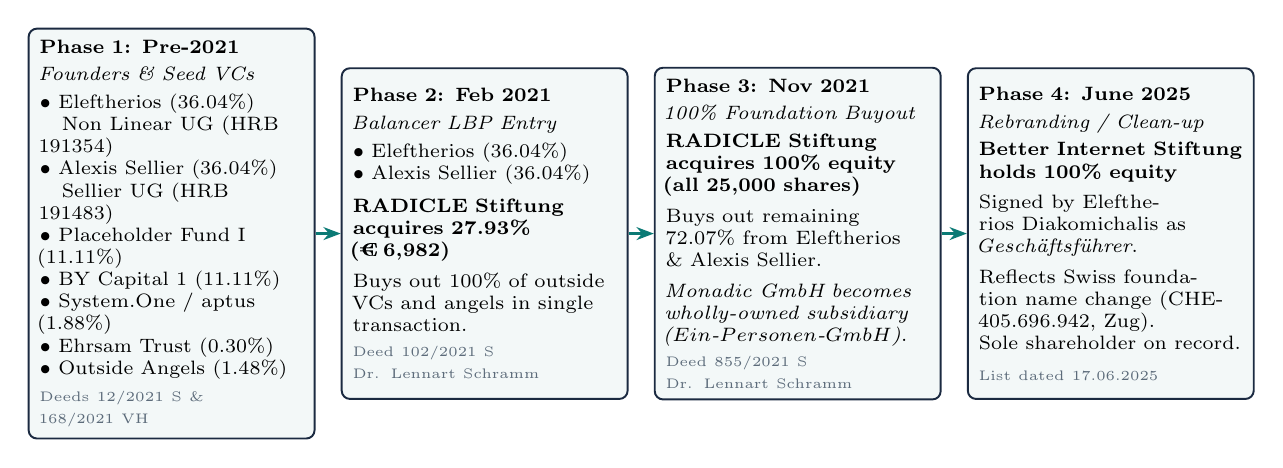
\begin{tikzpicture}[
  stage/.style={draw=ink, fill=accent!5, rounded corners=3pt, line width=0.7pt,
                text width=3.35cm, minimum height=4.2cm, align=left, font=\scriptsize, inner sep=4pt},
  arrow/.style={-{Stealth[length=2.2mm]}, line width=0.8pt, draw=accent}
]
  \node[stage] (p1) {\textbf{Phase 1: Pre-2021}\\[2pt]
    \emph{Founders \& Seed VCs}\\[2pt]
    $\bullet$ Eleftherios (36.04\%)\\
    \quad Non Linear UG (HRB 191354)\\
    $\bullet$ Alexis Sellier (36.04\%)\\
    \quad Sellier UG (HRB 191483)\\
    $\bullet$ Placeholder Fund I (11.11\%)\\
    $\bullet$ BY Capital 1 (11.11\%)\\
    $\bullet$ System.One / aptus (1.88\%)\\
    $\bullet$ Ehrsam Trust (0.30\%)\\
    $\bullet$ Outside Angels (1.48\%)\\[2pt]
    \tiny\color{mute} Deeds 12/2021~S \& 168/2021~VH};
  \node[stage, right=0.32cm of p1] (p2) {\textbf{Phase 2: Feb 2021}\\[2pt]
    \emph{Balancer LBP Entry}\\[2pt]
    $\bullet$ Eleftherios (36.04\%)\\
    $\bullet$ Alexis Sellier (36.04\%)\\[4pt]
    \textbf{RADICLE Stiftung}\\
    \textbf{acquires 27.93\% (\EUR{6{,}982})}\\[3pt]
    Buys out 100\% of outside VCs and angels in single transaction.\\[3pt]
    \tiny\color{mute} Deed 102/2021~S\\Dr. Lennart Schramm};
  \node[stage, right=0.32cm of p2] (p3) {\textbf{Phase 3: Nov 2021}\\[2pt]
    \emph{100\% Foundation Buyout}\\[2pt]
    \textbf{RADICLE Stiftung}\\
    \textbf{acquires 100\% equity}\\
    \textbf{(all 25{,}000 shares)}\\[3pt]
    Buys out remaining 72.07\% from Eleftherios \& Alexis Sellier.\\[3pt]
    \emph{Monadic GmbH becomes wholly-owned subsidiary ($Ein\text{-}Personen\text{-}GmbH$)}.\\[3pt]
    \tiny\color{mute} Deed 855/2021~S\\Dr. Lennart Schramm};
  \node[stage, right=0.32cm of p3] (p4) {\textbf{Phase 4: June 2025}\\[2pt]
    \emph{Rebranding / Clean-up}\\[2pt]
    \textbf{Better Internet Stiftung}\\
    \textbf{holds 100\% equity}\\[3pt]
    Signed by Eleftherios Diakomichalis as \emph{Geschäftsführer}.\\[3pt]
    Reflects Swiss foundation name change (CHE-405.696.942, Zug).\\
    Sole shareholder on record.\\[3pt]
    \tiny\color{mute} List dated 17.06.2025};
  \draw[arrow] (p1) -- (p2);
  \draw[arrow] (p2) -- (p3);
  \draw[arrow] (p3) -- (p4);
\end{tikzpicture}
\caption{The 4-phase cap table evolution of Monadic GmbH (Amtsgericht Charlottenburg, HRB 192171~B).}
\label{fig:captable_evolution}
\end{figure}

The notarized shareholder lists (\emph{Gesellschafterlisten}) establish the factual legal timeline:
\begin{enumerate}[nosep]
  \item \textbf{Pre-Token / Early Investors (Lists dated Jan 12, 2021 and Jan 28, 2021):} Co-founders Eleftherios Diakomichalis (via Non Linear Ventures UG) and Alexis Sellier (\code{cloudhead}, via Alexis Sellier Ventures UG) each held exactly 36.036\% (\EUR{9{,}009.00} nominal value each). Outside VC syndicates held 27.928\% (\EUR{6{,}982.00}), comprising Placeholder Fund~I (11.112\%), BY Capital 1 (11.112\%), System.One / aptus (1.876\%), Ehrsam Trust (0.300\%), Notation Capital (1.504\%), Neu LLC (1.504\%), and angels (UR-Nr. 12/2021~S, Notar Tobias Fuhrmann; UR-Nr. 168/2021~VH, Notar Dr.~Michael von Hinden).
  \item \textbf{The LBP Token Launch Shift (List dated Feb 24, 2021 --- Roll of Deeds 102/2021~S):} Coinciding with the Balancer LBP token launch in February 2021, the \textbf{RADICLE Stiftung} (Zug, CHE-405.696.942) entered the cap table. Notarized by Dr.~Lennart Schramm, the Foundation acquired all 6,982 shares (27.928\%) previously held by outside VCs and angels in a single buyout. Co-founders retained 36.036\% each.
  \item \textbf{Total Founder Buyout and Consolidation (List dated Nov 26, 2021 --- Roll of Deeds 855/2021~S):} Nine months later, RADICLE Stiftung acquired 100\% (all 25,000 shares) of Monadic GmbH. Eleftherios Diakomichalis and Alexis Sellier executed a complete share assignment of their remaining 72.072\% equity. Monadic GmbH became a wholly-owned subsidiary (\emph{Ein-Personen-GmbH}).
  \item \textbf{Rebranding and Governance Clean-up (List dated June 17, 2025):} Executed by Eleftherios Diakomichalis as sole \emph{Gesch{\"a}ftsf{\"u}hrer}: formally registers the Swiss parent's statutory name change to \textbf{Better Internet Stiftung} (CHE-405.696.942), confirming its unbroken 100\% ownership.
\end{enumerate}

\clearpage

\subsubsection{The Cargo-Cult ``Ethereum Foundation'' Blueprint: Legal Arbitrage and the German Tax Wall}
\label{sec:cargo_cult_blueprint}

Between 2017 and 2021, boutique corporate law firms in Zurich, Zug, and Berlin billed seven-figure retainers marketing an identical blueprint to crypto founders. The rationale---and why it deteriorated into severe balance-sheet liability---stems from jurisdictional legal arbitrage, conflicting tax regimes, and venture capital liquidity demands:

\begin{enumerate}[nosep]
  \item \textbf{The Cargo-Cult ``Ethereum Foundation'' Blueprint:} Copying Ethereum's 2014 Zug non-profit foundation (\emph{Stiftung}), founders treated Zug as an offshore liability shield against BaFin and the SEC: Swiss foundations are ownerless, purpose-bound entities overseen by the ESA, and pre-MiCA FINMA issued early ``no-action'' letters classifying utility tokens outside securities prospectuses. Founders replicated this structure uncritically to issue tokens without prospectus requirements.
  
  \item \textbf{The German Tax Wall \& VC Buyout (Why the GmbH was Sold):} Monadic GmbH (HRB 192171~B, Berlin 2018) hit a statutory wall when launching \$RAD in 2021: directly selling 100M tokens from Berlin was taxed as ordinary corporate income at $\approx$30\% (\emph{KSt + GewSt}), while early VCs demanded liquid tokens for illiquid GmbH equity. Corporate lawyers engineered a two-stage buyout:
  \begin{itemize}[nosep]
    \item \emph{Feb 2021 (LBP Token Sale \& VC Buyout):} RADICLE Stiftung (Zug) raised tens of millions offshore in the Balancer LBP, using proceeds to buyout 100\% of outside VC/angel equity (27.93\%, Roll of Deeds 102/2021~S).
    \item \emph{Nov 2021 (Founder Buyout):} The Foundation bought out founders Eleftherios and Alexis Sellier's remaining 72.07\% equity (Deed 855/2021~S), converting Monadic GmbH into a wholly-owned subsidiary (\emph{Ein-Personen-GmbH}) billing engineering hours upward.
  \end{itemize}

  \item \textbf{Why the Architecture Deteriorated:} Viable only during a temporary zero-interest bull market, the model produced three fatal structural liabilities once conditions normalized:
  \begin{itemize}[nosep]
    \item \emph{A. Dev Shop Legal Fiction:} A 100\%-owned subsidiary is not an independent third party, but a \emph{Konzerngesellschaft} (\S~15 AktG). Under MiCA Recital~22 (\emph{Substance over Form}), the veil dissolved: directors, management, and code repos sat in Berlin.
    \item \emph{B. Unfunded Intercompany Claim (\EUR{6.70M}):} Monadic carried \EUR{6.70M} in uncollected shareholder receivables (\emph{Forderungen gegen{\"u}ber Gesellschaftern}) against an upstream parent whose liquid USDC fell to $\sim$\$319k, backed by 40.9M illiquid \$RAD---creating instant write-down and insolvency under \S~253 Abs.~4 HGB and \S~19 InsO.
    \item \emph{C. Governance Illusion:} Decentralized DAO governance was an illusion: a single 3-signer contributor Safe held 7.11M unvested \$RAD (177\% of the 4M quorum) to unilaterally pass votes like RGP-29.
  \end{itemize}
\end{enumerate}

\begin{keybox}{The Underlying Incentive Structure: Why the Setup Persisted}
\begin{itemize}[nosep]
  \item \textbf{Law Firms:} Billed continuous seven-figure retainers maintaining dual Zug--Berlin entities.
  \item \textbf{Early VCs:} Secured an offshore liquidity path, converting illiquid equity into cash and liquid tokens.
  \item \textbf{Foundation \& Founders:} Maintained Berlin operations on token grants under a Swiss trust shield.
\end{itemize}
\end{keybox}

Post-MiCA, the 2021 middle ground---pretending to be an offshore Swiss non-profit on paper while operating a wholly-owned GmbH out of Kreuzberg---is permanently extinguished. The ecosystem has no choice: they are too late to pull out now via jurisdictional flight, and their sole survival path is to properly restructure, empower tokenholders, and build an on-chain economic sink for the token.

\clearpage

\subsubsection{Monadic GmbH Balance Sheet: The \EUR{6.70M} Shareholder Receivable Bomb}
\label{sec:monadic_balance_sheet_bomb}

The corporate root of the ecosystem is Monadic GmbH (HRB 192171 B, founded in Berlin in 2018). Whether operations remain formally in the GmbH or are shifted to Swiss foundations (The Better Internet Foundation for Radicle, Public Goods Association for Drips), the published annual balance sheet (\emph{Jahresabschluss zum 31.12.2023}, established March 31, 2025) exposes an acute structural exposure:

\begin{table}[H]
\centering\small
\renewcommand{\arraystretch}{1.06}
\begin{tabularx}{\textwidth}{@{}L{5.8cm} r r >{\RaggedRight\arraybackslash}X@{}}
\toprule
\textbf{Balance Sheet Position} & \textbf{31.12.2023} & \textbf{31.12.2022} & \textbf{Structural Ratio / Significance} \\
\midrule
\multicolumn{4}{@{}l@{}}{\textit{\textbf{Aktiva (Assets)}}} \\
\textbf{Fixed Assets} (\emph{Anlagevermögen}) & \EUR{33{,}679.43} & \EUR{37{,}624.43} & 0.44\% of assets; negligible tangible capital \\
\textbf{Current Assets} (\emph{Umlaufvermögen}) & \EUR{7{,}527{,}282.62} & \EUR{7{,}739{,}629.70} & 99.55\% of balance sheet total \\
\quad -- Trade \& other receivables & \EUR{7{,}493{,}520.81} & \EUR{7{,}566{,}271.57} & 99.11\% of current assets \\
\quad -- \textbf{Shareholder receivables} & \textbf{\EUR{6{,}697{,}240.35}} & \textbf{\EUR{6{,}740{,}679.78}} & \textbf{88.58\% of total assets (unhedged)} \\
\quad -- Cash \& bank deposits & \EUR{33{,}761.81} & \EUR{173{,}358.13} & Liquid cash reserves: \EUR{33.8k} (0.45\%) \\
\textbf{Total Assets (\emph{Bilanzsumme})} & \textbf{\EUR{7{,}560{,}962.05}} & \textbf{\EUR{7{,}777{,}254.13}} & \textbf{100.00\% of balance sheet total} \\
\midrule
\multicolumn{4}{@{}l@{}}{\textit{\textbf{Passiva (Equity \& Liabilities)}}} \\
\textbf{Equity} (\emph{Eigenkapital}) & \textbf{\EUR{5{,}403{,}551.06}} & \textbf{\EUR{5{,}315{,}029.08}} & Eradicated if shareholder claim impaired \\
Provisions (\emph{Rückstellungen}) & \EUR{2{,}084{,}260.04} & \EUR{2{,}409{,}060.06} & Contingent tax and operational reserves \\
Liabilities (\emph{Verbindlichkeiten}) & \EUR{73{,}150.95} & \EUR{53{,}164.99} & Short-term third-party liabilities ($<1$\,yr) \\
\textbf{Total Equity \& Liabilities} & \textbf{\EUR{7{,}560{,}962.05}} & \textbf{\EUR{7{,}777{,}254.13}} & \textbf{Balances Aktiva exactly (\S~266 HGB)} \\
\bottomrule
\end{tabularx}
\caption{Audited balance sheet of Monadic GmbH (HRB 192171 B, March 31, 2025). Shareholder receivables represent 88.58\% of total assets, creating acute upstream exposure.}
\label{tab:monadic_balance_sheet}
\end{table}

\begin{keybox}{Audited Statutory Disclosures (\emph{Anhang zum Jahresabschluss 2023}, Monadic GmbH)}
\begin{itemize}[nosep]
  \item \textbf{RAD Realization Dependency:} \emph{``Die sonstigen Erträge stammen überwiegend aus dem Verkauf bzw. der Realisierung von RAD Token.''} (Revenues derive predominantly from \$RAD token sales).
  \item \textbf{Trade Nature of Shareholder Debt:} \emph{``Die Forderungen gegen die Gesellschafter sind in Höhe von 6.686.866,72 Euro unter den Forderungen aus Lieferungen und Leistungen ausgewiesen.''} (\EUR{6.69M} billed to upstream DAO).
  \item \textbf{Personnel Relocation:} \emph{``Die Zahl der im Unternehmen beschäftigten Arbeitnehmer betrug 1.''} (Berlin GmbH formal workforce reduced to 1 employee).
\end{itemize}
\end{keybox}

\clearpage

\subsubsection{Legal Reality: Deconstructing the ``Gesellschafter-Forderung'' under \S~266 HGB}
\label{sec:deconstructing_forderung}

The notarized shareholder lists provide unambiguous legal clarity regarding the nature of the \textbf{\EUR{6.70M}} asset on Monadic GmbH's balance sheet (\cref{tab:monadic_balance_sheet}):
\begin{itemize}[nosep]
  \item Under German commercial accounting (\S~266 Abs.~2 B.II.2 HGB), the line item \emph{``Forderungen gegen{\"u}ber Gesellschaftern''} (Receivables from Shareholders) refers specifically and exclusively to claims owed by an entity listed on the formal commercial register \emph{Gesellschafterliste}.
  \item Since November 26, 2021, Monadic GmbH has had \textbf{exactly one shareholder}: the Better Internet Stiftung (f/k/a Radicle Stiftung, CHE-405.696.942, Zug).
  \item Consequently, the \textbf{\EUR{6{,}697{,}240.35}} balance-sheet claim (of which \EUR{6{,}686{,}866.72} is explicitly designated in statutory notes as trade receivables from services rendered) is a \textbf{direct legal intercompany liability of the Swiss Foundation}.
\end{itemize}
Monadic GmbH engineered core protocols in Berlin, billed \EUR{6.70M} upward to its Swiss parent entity, and carried the uncollected invoices on its Berlin balance sheet as an asset rather than drawing down liquid reserves.

\subsubsection{The Structural Dilemma: Monadic GmbH vs. Monadic Works GmbH}
\label{sec:monadic_works_dilemma}

The vulnerability of this arrangement is heightened by corporate restructuring in Berlin. On December 3, 2025, Eleftherios Diakomichalis founded a new corporate entity: \textbf{Monadic Works GmbH} (Amtsgericht Charlottenburg, HRB 283525~B):

\begin{figure}[H]
\centering
\vspace{-4pt}
\begin{tikzpicture}[
  box/.style={draw=ink, rounded corners=3pt, line width=0.7pt, align=left, font=\scriptsize, inner sep=3.5pt},
  arrow/.style={-{Stealth[length=2.0mm]}, line width=0.8pt}
]
  \node[box, fill=accent!8, text width=11.2cm] (parent) {
    \textbf{Better Internet Stiftung} (Zug, Switzerland -- CHE-405.696.942)\\[1pt]
    $\bullet$ Assets: Radworks DAO grant allocations \& illiquid \$RAD \quad $\bullet$ Timelock liquid USDC: $\sim$\$319k (RGP-28)
  };
  \node[box, fill=warn!8, below=0.45cm of parent, xshift=-3.4cm, text width=5.2cm] (old) {
    \textbf{Monadic GmbH (Old HRB 192171~B)}\\[1pt]
    $\bullet$ 100\% Swiss Foundation subsidiary; cash: \EUR{33.8k}\\
    $\bullet$ \textbf{Receivable: \EUR{6.70M} from Stiftung}\\
    $\bullet$ Managing Director: Eleftherios\\
    $\bullet$ \textbf{Insolvency trap: \S~253 Abs.~4 HGB \& \S~19 InsO}
  };
  \node[box, fill=accent!5, below=0.45cm of parent, xshift=3.4cm, text width=5.2cm] (new) {
    \textbf{Monadic Works GmbH (New HRB 283525~B)}\\[1pt]
    $\bullet$ Founded Dec 3, 2025 by Eleftherios\\
    $\bullet$ Fresh contributor contracts \& operational vehicle\\
    $\bullet$ \textbf{Tax trap: \S~1 Abs.~3b AStG}\\
    $\bullet$ \textbf{Clawback trap: \S~826 BGB \& InsO}
  };
  \draw[arrow, draw=warn] (parent.south -| old.north) -- node[left, font=\tiny\bfseries, text=warn, align=right] {100\% Equity /\\\EUR{6.70M} Claim} (old.north);
  \draw[arrow, dashed, draw=mute] (old.east) -- node[above=1pt, font=\tiny, text=mute, align=center] {Transfer of\\functions?} (new.west);
\end{tikzpicture}
\vspace{-6pt}
\caption{The structural dilemma: legacy balance-sheet liabilities in Monadic GmbH vs. Monadic Works GmbH.}
\label{fig:monadic_works_split}
\end{figure}

Founding an unencumbered vehicle in late 2025 to route fresh contributor contracts and operational disbursements while stranding legacy balance-sheet liabilities creates two severe statutory exposures:
\begin{enumerate}[nosep]
  \item \textbf{The Capital Maintenance Trap (\S~30 GmbHG \& \S~253 Abs.~4 HGB):} Monadic GmbH's \EUR{6.70M} receivable depends on Better Internet Stiftung, whose liquid DAO Timelock was reduced to $\sim$\$319k USDC in RGP-28, backed by 40.9M illiquid \$RAD. Inability to satisfy the claim in cash triggers mandatory write-downs under \S~253 Abs.~4 HGB, wiping out \EUR{5.40M} equity and creating statutory over-indebtedness (\emph{{\"U}berschuldung}, \S~19 InsO).
  \item \textbf{The Transfer-of-Functions Trap (\S~1 Abs.~3b AStG \& \S~826 BGB):} Migrating operational assets, contributor workflows, or IP from Monadic GmbH to Monadic Works GmbH without arm's-length cash compensation is treated by the \emph{Finanzamt} as a taxable Transfer of Functions (\emph{Funktionsverlagerung}, \S~1 Abs.~3b AStG). Subsequent insolvency of Monadic GmbH triggers clawback actions (\S\S~133, 134 InsO) and corporate veil-piercing under \S~826 BGB (\emph{existenzvernichtender Eingriff}).
\end{enumerate}

\clearpage

\subsubsection{The Dual Statutory Exposure: Mandatory Insolvency vs. Capital Maintenance}
\label{sec:monadic_dual_exposure}

This balance-sheet structure exposes the entity and its management to two acute legal traps under German statutory law:

\begin{warnbox}{Trap A: Mandatory Write-Down and Balance-Sheet Insolvency (\S~253 Abs.~4 HGB \& \S~19 InsO)}
\textbf{The Statutory Rule:} Under \S~253 Abs.~4 HGB (\emph{strenges Niederstwertprinzip}), current receivables must be written down immediately if there is any foreseeable risk of non-collection.
\begin{itemize}[nosep]
  \item \textbf{Exhaustion of Liquid Reserves:} Prior to December 2025, the upstream DAO held millions in liquid USDC. Following RGP-28, the DAO Timelock disbursed \$2.994M USDC to Swiss entities, leaving just \textbf{\$319,133 USDC} alongside 40.92M illiquid \$RAD.
  \item \textbf{Un-liquidatable Collateral:} Because 40.92M \$RAD represents 40.9\% of total supply and decentralized pool depth is less than 1.5\% of reported CEX volume, the debtor cannot convert \$RAD into cash without crashing spot prices by 80--90\%. The debtor is factually unable to satisfy a \EUR{6.70M} cash demand.
  \item \textbf{Instant Over-Indebtedness (\emph{Überschuldung}):} An auditor requiring even a 50\% impairment (\EUR{3.35M}) wipes out 62\% of Monadic GmbH's \EUR{5.40M} equity. A full write-down leaves negative equity of \EUR{-1.30M}, triggering statutory balance-sheet over-indebtedness under \S~19 InsO.
  \item \textbf{Insolvency Filing Deadline (\S~15a InsO):} Managing directors (\emph{Geschäftsführer}) have a strict statutory window of 3 to 6 weeks to file for insolvency upon over-indebtedness. Delayed filing constitutes \emph{Insolvenzverschleppung}, resulting in unlimited personal civil liability (\S~43 GmbHG) and criminal sanctions (\S~15a Abs.~4 InsO).
\end{itemize}
\end{warnbox}

\begin{warnbox}{Trap B: Swiss Evacuation Tax Bomb and Capital Maintenance (\S~1 Abs.~3b AStG \& \S~30 GmbHG)}
\textbf{The Statutory Rule:} Under German corporate law, a Berlin GmbH cannot gift technology, forgive shareholder debt, or transfer ongoing operations without arm's-length cash compensation.
\begin{itemize}[nosep]
  \item \textbf{Capital Maintenance Violation (\S~30 GmbHG -- \emph{Verbot der Einlagenrückgewähr}):} Forgiving, waiving, or failing to strictly enforce the \EUR{6.70M} shareholder claim is an illegal return of capital. Under \S~30 Abs.~1 Satz~2 GmbHG, shareholder receivables must be fully recoverable (\emph{vollwertig}) at all times. Under \S~43 Abs.~3 GmbHG, managing directors are personally liable with their entire private wealth to reimburse the GmbH.
  \item \textbf{Transfer of Functions Tax (\emph{Funktionsverlagerung}, \S~1 Abs.~3b AStG):} Migrating protocol development to Swiss non-profits (The Better Internet Foundation for Radicle Garden and Public Goods Association for Drips) while leaving \EUR{6.70M} in receivables uncollected triggers an automatic statutory transfer-of-functions assessment.
  \item \textbf{Hidden Profit Distribution (\emph{vGA}, \S~8 Abs.~3 Satz~2 KStG):} The Berlin \emph{Finanzamt} treats the transferred software business and waived receivables as a hidden distribution of profit, assessing $\approx$30\% corporate/trade tax (\emph{KSt + GewSt}) plus 25\% capital yields withholding tax in immediate cash that the GmbH does not possess.
\end{itemize}
\end{warnbox}

\clearpage

\subsubsection{The Insolvency Administrator's Audit: Lugano Convention, Clawbacks, and Criminal Delay}
\label{sec:insolvency_administrator_audit}

In German insolvency proceedings, the corporate veil does not merely slip---the court-appointed insolvency administrator (\emph{Insolvenzverwalter}) is statutorily mandated to dismantle it. Under the German Insolvency Statute (\emph{Insolvenzordnung} -- InsO), the administrator represents neither the founder, the board, nor the Swiss parent; their exclusive legal duty is to maximize cash recovery for the creditor pool (\emph{Gl{\"a}ubigergesamtheit}). A formal petition over Monadic GmbH triggers a multi-front cross-border liquidation:
\begin{enumerate}[nosep]
  \item \textbf{Immediate Loss of Operational Control (\S~80 InsO):} The managing director is instantly stripped of all managerial and dispositional authority (\emph{Verwaltungs- und Verf{\"u}gungsbefugnis}). The administrator seizes all corporate bank accounts, physical offices, contributor contracts, source repository credentials, and accounting databases.
  \item \textbf{Cross-Border Enforcement under the Lugano Convention (\emph{Lug{\"U}}):} Finding \EUR{6.70M} in receivables against the sole shareholder (Better Internet Stiftung, Zug), the administrator issues an immediate formal demand for payment. Under the Lugano Convention on Jurisdiction and the Recognition and Enforcement of Judgments (\emph{Lugano-{\"U}bereinkommen} -- Lug{\"U}), German insolvency judgments and payment orders are directly enforceable in Switzerland through the debt collection office (\emph{Betreibungsamt Zug}). Because the Swiss Foundation holds only $\sim$\$319k in liquid USDC alongside 40.9M illiquid \$RAD that cannot be liquidated on-chain without an 80--90\% price crash, the Swiss Foundation is forced into involuntary Swiss bankruptcy proceedings (\emph{Konkursverfahren} under the \emph{Bundesgesetz {\"u}ber Schuldbetreibung und Konkurs} -- SchKG).
  \item \textbf{Monadic Works Clawback Actions (\S\S~129 ff. InsO):} The incorporation of Monadic Works GmbH on December 3, 2025 across the same hallway in Berlin creates acute clawback exposure:
  \begin{itemize}[nosep]
    \item \emph{Intentional Detriment (\S~133 InsO -- Vorsatzanfechtung):} If contributor workflows, service agreements, or client subscriptions were shifted to Monadic Works while Monadic GmbH carried unhedged balance-sheet liabilities, the administrator has a multi-year statutory lookback window to retroactively void and claw back all transferred assets, operational goodwill, and diverted revenue streams.
    \item \emph{Gratuitous Transfers (\S~134 InsO -- Schenkungsanfechtung):} Any migration of source code, tooling, or infrastructure without an audited, arms-length cash purchase price (\emph{Fremdvergleich}) is statutorily voided and reclaimed for the bankruptcy estate.
    \item \emph{Destruction of Corporate Existence (\S~826 BGB -- Existenzvernichtender Eingriff):} Under established Federal Court of Justice (\emph{Bundesgerichtshof} -- BGH) jurisprudence, stripping operational substance from an operating GmbH while stranding an uncollectible receivable against an offshore parent constitutes intentional immoral injury to creditors (\emph{vors{\"a}tzliche sittenwidrige Sch{\"a}digung}), piercing the corporate veil to impose unlimited, joint personal civil liability on managing and shadow directors.
  \end{itemize}
  \item \textbf{Personal Criminal Liability for Insolvency Delay (\S~15a InsO \& \S~283 StGB):} A statutory going-concern forecast (\emph{positive Fortf{\"u}hrungsprognose}) cannot legally rely on speculative future token appreciation. Writing down the uncollectible Swiss receivable under \S~253 Abs.~4 HGB creates instantaneous balance-sheet over-indebtedness. Exceeding the strict statutory filing window triggers criminal prosecution for insolvency delay (\emph{Insolvenzverschleppung}, \S~15a Abs.~4 InsO) and bankruptcy fraud (\emph{Bankrott}, \S~283 StGB).
  \item \textbf{Regulatory Evidentiary Spillover into BaFin and ESMA:} In an insolvency proceeding, all corporate filings, token sale records, and governance correspondence become court records. The administrator's forensic audit delivers unredacted documentation directly to BaFin and ESMA, cementing enforcement actions under MiCA Article~111 and the German KMAG.
\end{enumerate}

\subsubsection{Dissolution of the Corporate Veil: Single Economic Entity (\emph{Konzern}) under MiCA and KMAG}
\label{sec:corporate_veil_dissolution}

The structure exposed in the official \emph{Gesellschafterlisten} dissolves the affirmative defense historically relied upon by Web3 organizations under European financial regulation. For years, projects operated under a two-tier organizational narrative:
\begin{quote}
\emph{``The token was issued by an independent non-profit foundation in Zug (CHE-405.696.942); the Berlin GmbH is merely an independent service contractor billing for engineering hours.''}
\end{quote}
Having 100\% of Monadic GmbH owned by the Better Internet Stiftung completely invalidates that defense under MiCA and German administrative law:

\begin{enumerate}
  \item \textbf{A Single Economic Entity (\emph{Konzern}):} Under German company law and European corporate governance, an entity whose shares are 100\% held by a Swiss parent is not an independent contractor---it is a wholly-owned subsidiary (\emph{Konzernunternehmen} under \S~15 et seq. AktG by analogy). Under MiCA Recital~22, the European Securities and Markets Authority (ESMA) and national competent authorities enforce the doctrine of \textbf{Substance over Form} (\emph{Substanz vor Form}): regulators evaluate which physical persons and corporate organs exercise discretionary control over infrastructure, token distribution, and governance. The Swiss Foundation owns 100\% of Monadic GmbH; the sole managing director of Monadic GmbH (Eleftherios Diakomichalis) directs operations from Berlin; and the Berlin GmbH carries a \EUR{6.70M} receivable against its Swiss owner while acknowledging in its statutory notes that its revenues derive from selling and realizing \$RAD tokens. To BaFin and ESMA, the Swiss foundation is not an untouchable offshore trust---Monadic GmbH in Berlin is the domestic EU operational establishment of the token issuer/offeror.
  \item \textbf{The MiCA Title~II and Third-Country Issuer Trap:} Because Better Internet Stiftung is domiciled in Zug, Switzerland (a non-EU third country):
  \begin{itemize}
    \item \emph{No Reverse Solicitation Defense (MiCA Article~61):} A third-country entity cannot actively promote, distribute, or service crypto-assets to EU users without authorization unless the client initiated the transaction on their own exclusive initiative. That exception collapses when an active EU subsidiary develops the software, operates hosted front-ends, and liquidates tokens onshore.
    \item \emph{The ``Offeror'' Requirement (MiCA Articles~4 \& 5):} Under Article~4(1), offering a crypto-asset (other than ARTs/EMTs) to the public in the Union requires a legal person and an approved, published whitepaper.
    \item \emph{Domestic Enforcement Anchor:} When European authorities sanction an unregistered third-country issuance or demand statutory disclosures, they do not need to deal with Swiss mutual legal assistance treaties. Under the German \emph{Kryptom{\"a}rkteaufsichtsgesetz} (KMAG), BaFin enforces directly against the registered EU entity on Gneisenaustra{\ss}e in Berlin. Under MiCA Article~111, corporate fines can reach \EUR{5{,}000{,}000} or 3\% to 5\% of annual turnover, alongside personal director liability.
  \end{itemize}
  \item \textbf{Front-End Intermediary Liability Under ESMA Guidelines:} ESMA's regulatory guidance for decentralized finance establishes that web interfaces and hosted services managed by identifiable corporate entities trigger intermediary status:
  \begin{itemize}
    \item The ecosystem operates \code{radicle.garden} as a commercial hosted service charging users subscription fees (\EUR{4.99}/month).
    \item In the published legal terms and privacy disclosures for \code{radicle.garden}, Monadic GmbH is explicitly listed as a joint data controller.
  \end{itemize}
  The same Berlin entity that built the code and holds a \EUR{6.70M} debt against the token-funded foundation serves as the administrative front-end for end-users. Claiming the network is an autonomous, un-regulatable public utility is legally untenable when user traffic routes through an interface managed by a 100\%-owned subsidiary in Berlin.
\end{enumerate}

\subsubsection{Statutory Liability Refinements: \S~54 Abs.~2 BGB, \S\S~705, 721 BGB, and GDPR Continuity}
\label{sec:bgb_liability_gdpr}

Under German conflict of laws (\emph{Sitztheorie}), an unincorporated foreign DAO whose key founders, contributors, and core developers operate out of Berlin is classified as an \emph{Außen-GbR} (civil law partnership) or a \emph{nichtrechtsfähiger Verein}:
\begin{itemize}[nosep]
  \item \textbf{Personal Joint Liability (\S~54 Abs.~2 BGB \& \S~721 BGB):} Anyone acting on behalf of the DAO incurs direct, unlimited, and joint personal liability (\emph{persönliche und gesamtschuldnerische Haftung}).
  \item \textbf{Corporate Continuity \& GDPR Controller Admission:} While ecosystem communications suggest complete operational separation into Swiss non-profits, the live Privacy Policy of Radicle Garden (\path{radicle.garden/privacy}, updated February 2026) explicitly designates Monadic GmbH as a joint GDPR controller, proving unbroken operational continuity in Berlin.
\end{itemize}

\subsubsection{Market Telemetry: The October 5, 2026 Surge and the December 2026 Runway Cliff}
\label{sec:october_telemetry_cliff}

On October 5, 2026, market telemetry highlighted the disconnect between secondary exchange activity and on-chain protocol utility:
\begin{itemize}
  \item \$RAD surged +32.03\% in 24 hours (from \$0.2614 to \$0.3451), registering \$61.70 million in reported centralized exchange (CEX) volume---a 24-fold increase over its 30-day baseline.
  \item However, on-chain decentralized liquidity (Uniswap V2) accounted for only \$950,600 (1.54\% of total volume), confirming that 98.46\% of trading was off-chain CEX churning driven by Turkish Lira (TRY) and Korean Won (KRW) speculative arbitrage. On October 6, 2026, Phemex delisted its \$RAD trading pairs.
  \item Every comparable volume spike over the prior 18 months (March 10, 2025; Dec 31, 2025; May 11, 2026; Aug 10, 2026) retraced entirely within 30 days due to the absence of an on-chain utility sink.
\end{itemize}
At the close of 2026, three deadlines converge:
\begin{enumerate}
  \item The 2026 USDC budgets from RGP-28 expire, leaving only \$319k in liquid stablecoins in the DAO Timelock.
  \item The 7.11 million \$RAD held in the Drips Safe multisig reaches its December 2026 unlock cliff.
  \item Monadic GmbH closes its financial year on December 31, 2026, requiring accountants to verify whether the \EUR{6.70M} receivable remains solvent.
\end{enumerate}

\subsubsection{The Two Remaining Paths: Jurisdictional Flight (The IOTA / ADGM Playbook) vs. Technical Legitimization}
\label{sec:two_paths_iota_vs_legitimacy}

The historical middle ground that characterized the 2017--2021 crypto boom---maintaining an offshore Swiss foundation on paper while running an unhedged domestic development GmbH out of Berlin-Kreuzberg---is permanently extinguished under MiCA and German commercial law. Only two operational paths remain on the board:

\paragraph{Path 1: The Jurisdictional Flight (The IOTA / ADGM Playbook).}
A prominent German precedent is the IOTA ecosystem, which incorporated as a non-profit foundation in Berlin under the Berlin Foundation Authority (\emph{Stiftungsaufsicht Berlin}), endured years of regulatory friction and supervisory paralysis, and eventually fled to Abu Dhabi (ADGM) in 2023 to establish an offshore DLT foundation. However, attempting this flight post-MiCA encounters immediate statutory barriers under German and European law:
\begin{itemize}[nosep]
  \item \textbf{The German Liquidation Lock (\S~73 GmbHG -- \emph{Sperrjahr}):} A German GmbH cannot be abandoned or dissolved overnight. Statutory corporate liquidation (\emph{Abwicklung}) requires publishing a formal call to creditors (\emph{Gl{\"a}ubigeraufruf}) in the \emph{Federal Gazette} (\emph{Bundesanzeiger}), initiating a mandatory one-year waiting period (\emph{Sperrjahr}). During this year, liquidators remain personally liable with their entire private wealth for all corporate obligations. Because the \EUR{6.70M} shareholder claim cannot be converted into cash to extinguish outstanding tax, supplier, and operational liabilities, the entity cannot complete liquidation; the liquidator is legally compelled to file for insolvency under \S~15a InsO.
  \item \textbf{Exit Taxation (\S~6 AStG -- \emph{Wegzugsbesteuerung}):} If key management or controlling contributors relocate their tax residency outside the EU/EEA, the German \emph{Finanzamt} treats all unrealized company value, brand equity, and protocol IP appreciation as a deemed taxable liquidation sale, assessing immediate cash income tax without an underlying liquidity event.
  \item \textbf{The MiCA Article~61 Third-Country Barrier:} Relocating to Zug or Abu Dhabi fails to circumvent European jurisdiction. MiCA's third-country regime strictly prohibits actively servicing or marketing to EU users without an authorized domestic EU entity. If European developers access \code{radicle.garden} or run nodes within the Union, flight to an offshore jurisdiction fails to insulate management from BaFin enforcement.
  \item \textbf{Extinction of the Open-Source Ethos:} Fleeing to an offshore tax haven to operate an open-source code collaboration protocol destroys developer trust and fatally alienates the cypherpunk community.
\end{itemize}

\paragraph{Path 2: Dismantle the Arbitrage and Become Fully Legitimate.}
The only viable strategy is to do the hard, honest engineering work: dismantle the legal fictions, eliminate insider choke points, empower tokenholders, and align corporate, cryptographic, and economic reality:
\begin{enumerate}[nosep]
  \item \textbf{Audit and Settle Intercompany Debt:} Before the close of the 2026 fiscal year, the \EUR{6.70M} shareholder receivable must be converted into an audited, closed debt-settlement covenant or satisfied through legitimate treasury liquidity, eliminating \S~253 HGB write-down exposure and \S~19 InsO over-indebtedness.
  \item \textbf{Attain Genuine MiCA Recital 22 Technical Decentralization:} Anchor repository state in stateless CAR Slot~3 manifolds, verified by independent nodes running zero-knowledge SBOM proofs. Retire the 3-signer Safe multisig commanding 177\% of quorum in favor of verifiable TinyMeritRank merit consensus, transforming tokenholders from passive bystanders into sovereign protocol participants.
  \item \textbf{Anchor the Token in Real Economic Utility:} Transition \$RAD from an illiquid speculative asset on secondary exchanges into CAR Slot~8 Operational Surety Bonds. Deploy an automated EUR/RAD liquidity corridor in Europe to capture FX arbitrage, absorb floating supply, and provide predictable operating revenues for node operators and core maintainers.
\end{enumerate}

\subsubsection{The Structural Remedy: Corporate Hierarchy vs. Sovereign Mesh Architecture}
\label{sec:structural_remedy}

To resolve regulatory exposure under MiCA and eliminate balance-sheet insolvency risks under German corporate law, the ecosystem requires a definitive structural transition:

\begin{figure}[H]
\centering
\begin{tikzpicture}[
  pane/.style={draw=ink, rounded corners=4pt, line width=0.8pt, align=left, font=\small, inner sep=6pt, text width=7.0cm},
  subnode/.style={draw=mute, fill=white, rounded corners=2pt, line width=0.5pt, align=left, font=\scriptsize, inner sep=4pt, text width=6.2cm}
]
  % Left: Vulnerable Architecture
  \node[pane, fill=warn!5] (left) {
    \textbf{\color{warn}Vulnerable 2021--2026 Hierarchy}\\[4pt]
    \begin{tikzpicture}[node distance=0.55cm]
      \node[subnode, fill=warn!10] (z) {\textbf{Better Internet Stiftung (Zug)}\\$\bullet$ Domiciled in non-EU third country\\$\bullet$ Holds illiquid \$RAD; \$319k liquid USDC};
      \node[subnode, fill=warn!15, below=of z] (m) {\textbf{Monadic GmbH (Berlin, HRB 192171~B)}\\$\bullet$ 100\% subsidiary ($Konzern$ under \S~15 AktG)\\$\bullet$ Carries \EUR{6.70M} unbacked claim\\$\bullet$ BaFin / KMAG primary enforcement anchor\\$\bullet$ GDPR controller for \code{radicle.garden}};
      \draw[-{Stealth[length=2mm]}, line width=0.8pt, draw=warn] (z) -- node[right=2pt, font=\tiny\bfseries, text=warn, align=left] {100\% Equity /\\\EUR{6.7M} Claim} (m);
    \end{tikzpicture}
  };
  
  % Right: Sovereign Mesh Architecture
  \node[pane, fill=accent!5, right=0.5cm of left] (right) {
    \textbf{\color{accent}Sovereign Mesh Architecture}\\[4pt]
    \begin{tikzpicture}[node distance=0.55cm]
      \node[subnode, fill=accent!10] (mesh) {\textbf{Autonomous Open-Source Mesh}\\$\bullet$ Stateless CAR Slot~3 Git repo manifolds\\$\bullet$ Multi-seed TinyMeritRank consensus\\$\bullet$ Zero corporate intermediary (MiCA Recital 22)};
      \node[subnode, fill=accent!15, below=of mesh] (nodes) {\textbf{Independent Commercial Nodes}\\$\bullet$ Dispersed EU and global seed operators\\$\bullet$ Bound by Slot~8 Surety Bonds\\$\bullet$ Paid SLA streams; EUR/RAD liquidity corridor\\$\bullet$ Complete legal \& technical decentralization};
      \draw[-{Stealth[length=2mm]}, line width=0.8pt, draw=accent] (mesh) -- node[right=2pt, font=\tiny\bfseries, text=accent, align=left] {Peer Consensus /\\SLAs \& Bonds} (nodes);
    \end{tikzpicture}
  };
\end{tikzpicture}
\caption{Comparison: Vulnerable centralized corporate hierarchy versus polycentric Sovereign Mesh architecture.}
\label{fig:structural_remedy_comparison}
\end{figure}

This architectural transition provides an actionable path to regulatory compliance and balance-sheet continuity:
\begin{enumerate}
  \item \textbf{Sever the Operational Monopoly via CAR Slot~3:} Repository hosting and canonical reference consensus must move from corporate-hosted servers into stateless CAR Slot~3 manifolds. When repository verification is executed by independent third-party nodes running zero-knowledge SBOM proofs, the system satisfies the MiCA Recital~22 criterion for full technical decentralization.
  \item \textbf{Eliminate the 177\% Quorum Multisig via TinyMeritRank:} Governance cannot remain concentrated in an insider Safe multisig commanding 177\% of quorum. Transitioning to TinyMeritRank replaces token-weighted plutocracy with verifiable, relationship-native merit consensus, dismantling the single administrative point of failure targeted by regulatory bodies.
  \item \textbf{Resolve the \EUR{6.70M} Intercompany Claim via the EUR/RAD Corridor:} The \EUR{6.70M} shareholder receivable between Zug and Berlin must be settled before the 2026 fiscal year-end audit. Establishing a transparent EUR/RAD liquidity corridor (\cref{sec:bootstrap_corridor}) creates an orderly mechanism to convert token reserves into Euro-denominated collateral (EURe / CBMT), settling the balance-sheet exposure without destructive CEX dumping.
\end{enumerate}

\begin{figure}[H]
\centering
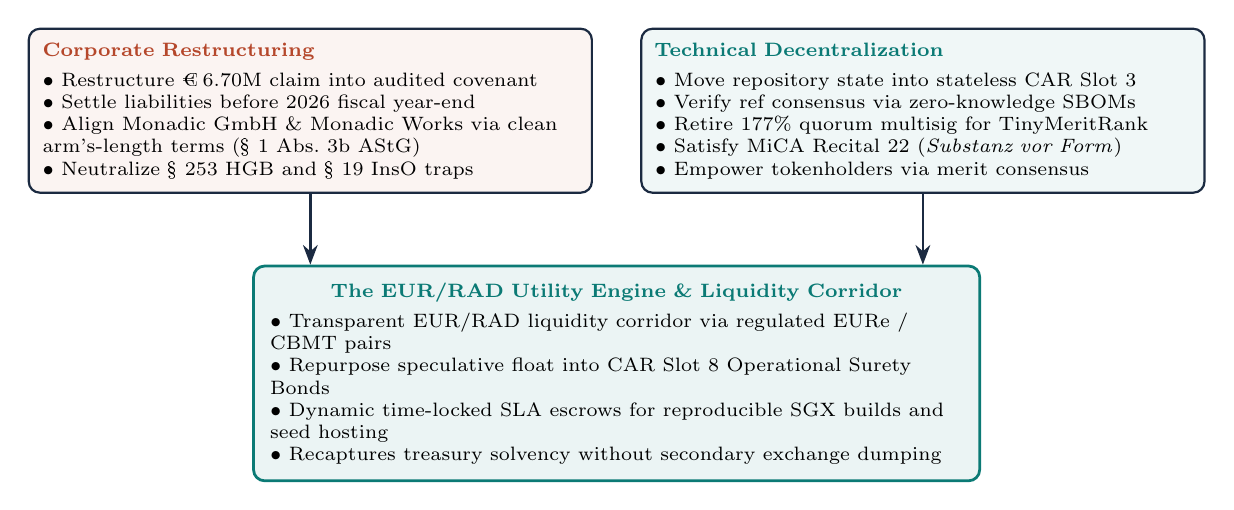
\begin{tikzpicture}[
  pane/.style={draw=ink, rounded corners=4pt, line width=0.8pt, align=left, font=\scriptsize, inner sep=5pt, text width=6.8cm},
  engine/.style={draw=accent, fill=accent!8, rounded corners=4pt, line width=1pt, align=left, font=\scriptsize, inner sep=6pt, text width=8.8cm},
  arrow/.style={-{Stealth[length=2.5mm]}, line width=0.9pt, draw=ink}
]
  % Top Left: Corporate Restructuring
  \node[pane, fill=warn!6] (corp) {
    \textbf{\color{warn}Corporate Restructuring}\\[3pt]
    $\bullet$ Restructure \EUR{6.70M} claim into audited covenant\\
    $\bullet$ Settle liabilities before 2026 fiscal year-end\\
    $\bullet$ Align Monadic GmbH \& Monadic Works via clean arm's-length terms (\S~1 Abs.~3b AStG)\\
    $\bullet$ Neutralize \S~253 HGB and \S~19 InsO traps
  };
  
  % Top Right: Technical Decentralization
  \node[pane, fill=accent!6, right=0.6cm of corp] (tech) {
    \textbf{\color{accent}Technical Decentralization}\\[3pt]
    $\bullet$ Move repository state into stateless CAR Slot~3\\
    $\bullet$ Verify ref consensus via zero-knowledge SBOMs\\
    $\bullet$ Retire 177\% quorum multisig for TinyMeritRank\\
    $\bullet$ Satisfy MiCA Recital~22 (\emph{Substanz vor Form})\\
    $\bullet$ Empower tokenholders via merit consensus
  };
  
  % Bottom Center: The EUR/RAD Engine
  \node[engine, below=0.9cm of $(corp.south)!0.5!(tech.south)$] (engine) {
    \centering\textbf{\color{accent}The EUR/RAD Utility Engine \& Liquidity Corridor}\\[3pt]
    \raggedright
    $\bullet$ Transparent EUR/RAD liquidity corridor via regulated EURe / CBMT pairs\\
    $\bullet$ Repurpose speculative float into CAR Slot~8 Operational Surety Bonds\\
    $\bullet$ Dynamic time-locked SLA escrows for reproducible SGX builds and seed hosting\\
    $\bullet$ Recaptures treasury solvency without secondary exchange dumping
  };
  
  \draw[arrow] (corp.south) -- ++(0,-0.35) -| (engine.north -| corp.south);
  \draw[arrow] (tech.south) -- ++(0,-0.35) -| (engine.north -| tech.south);
\end{tikzpicture}
\caption{The Cleanup and Legitimization Architecture: resolving corporate liabilities and achieving genuine MiCA Recital 22 decentralization through the Sovereign Mesh and EUR/RAD engine.}
\label{fig:cleanup_architecture}
\end{figure}

\subsection{Repurposing Legacy Float: From Governance Theater to Operational Surety Bonds}
\label{sec:repurposing_rad_float}

The traditional crypto-economic playbook relies on speculative governance tokens, which trigger regulatory scrutiny under MiCA and Howey while failing to support protocol operations. The Sovereign Bunny architecture establishes a different model: repurposing legacy liquid float (\$RAD) into \textbf{operational surety bonds} allocated within CAR Slot~8 ($R_8$).

Rather than leaving 40.92M \$RAD dormant in an illiquid timelock, tokens are deposited through the Mirrored Boundary Consensus precompile (\code{0x00...0002}) into single-writer account registers:
\begin{enumerate}
  \item \textbf{Canonical Namespace Bonding:} In a polycentric network, naming is local by default (\code{auth.cbase-ber}). To secure a canonical routing alias across the federated index, a seed node operator locks an operational bond in Slot~8.
  \item \textbf{Non-Equivocation Collateral:} If a seed operator signs two conflicting head references for the same Git ref, the signed split-DAG acts as a self-contained fraud proof, slashing the bonded Slot~8 tokens into the Protocol Insurance Reserve.
  \item \textbf{High-Assurance Relay Escrow:} Enterprise tenants commissioning continuous reproducible SGX builds or priority bandwidth pipes lock dynamic SLA escrows denominated in bridged \$RAD or Commercial Bank Money Tokens (CBMT-EUR).
\end{enumerate}

\subsection{The EUR/RAD Algorithmic Bootstrap Corridor and CEX Inventory Physics}
\label{sec:bootstrap_corridor}

Deploying a new token under MiCA entails extensive white paper approvals and regulatory overhead before achieving production scale. Utilizing an established legacy asset (\$RAD) within a bounded utility corridor avoids this barrier:
\begin{itemize}
  \item \textbf{The \EUR{1,000,000} Safe Harbor (MiCA Article~4(2)(a)):} Cross-chain experimental bonding operating under the rolling 12-month \EUR{1M} consideration threshold requires no public retail white paper or NCA approval while the protocol hardens its cryptographic kernel.
  \item \textbf{Multi-Hop Friction as Regulatory Armor:} Capital enters the execution mesh via deliberate, technical steps:
  \begin{equation}
    \text{Fiat (EUR)} \longrightarrow \text{Regulated CASP (RAD/ETH)} \longrightarrow \text{Self-Custodial Withdrawal} \longrightarrow \text{Low-Entropy Bridge (\code{0x02})} \longrightarrow \text{Stateless Mesh}
  \end{equation}
  Because participation requires intentional cryptographic bridge execution, the protocol operates beyond the custodial CASP perimeter. Regulators are insulated from retail impulse claims, and exchanges offload downstream execution liability.
  \item \textbf{CEX Inventory Squeeze and Balance-Sheet Solvency:} When node operators lock \$RAD into long-term canonical naming bonds and SLA escrows, float is withdrawn from centralized exchange omnibus wallets. As order books thin, institutional desks seeking inventory must enter direct, compliant OTC tranches with the ecosystem treasury. This generates verifiable fiat/USDC runway without dumping tokens into public automated market makers, establishing legitimate recoverability for Monadic GmbH's \EUR{6.70M} receivable under \S~253 HGB.
\end{itemize}

\subsection{Open-Hardware Symbiosis: From Code Commons to Physical BOMs}
\label{sec:hardware_symbiosis}

A pure software forge that relies exclusively on developer donations struggles to achieve long-term financial stability. Linking repository state in Slot~3 directly to open-hardware ecosystems (such as PINE64, InfiniTime, Wasp-OS, Gadgetbridge, and postmarketOS) provides a concrete operational foundation:
\begin{enumerate}
  \item \textbf{Crowdfunded Factory MOQs (Slots~4 \& 8):} Community batch runs of open-hardware terminals (such as low-power Memory-in-Pixel watches or edge nodes) pool pre-orders in Slot~8 escrows, funding factory Minimum Order Quantities (MOQs) directly without venture debt.
  \item \textbf{CRA and SLSA Level 3 Compliance:} The European Union's Cyber Resilience Act (CRA) mandates verifiable software bills of materials (SBOMs) for connected hardware by 2027. Radicle repository anchors in Slot~3 provide cryptographic provenance for hardware firmware.
  \item \textbf{The Betamax vs. VHS Precedent:} Restricting a protocol to a closed, pure environment risks isolation. By opening to network-scoped DIDs and integrating an automated EUR/RAD liquidity bridge, the ecosystem supports real economic transactions across hardware deployments, IoT vending, and code collaboration.
\end{enumerate}

\subsection{Sociological Foundations: Do-ocracy, Legal Firewalls, and the KDE Precedent}
\label{sec:kde_precedent}

The structural challenges facing Radicle mirror those of early open-source initiatives, notably the KDE desktop environment in 1996--1997. When KDE chose the Qt toolkit, the project faced ideological pushback over software licensing. The community resolved this not through prolonged debate, but through technical execution and clear legal structuring:
\begin{itemize}
  \item \textbf{Do-ocracy:} Operational decisions were driven by contributors writing code: \emph{``whoever does the work decides what gets done''}.
  \item \textbf{The Legal Firewall:} To remove counterparty risk, the community established the \textbf{KDE Free Qt Foundation} and \textbf{KDE e.V.}, legally guaranteeing that if the corporate entity failed or altered its terms, the core software would automatically relicense under open terms.
  \item \textbf{The KDE 4.0 Refactoring Moment:} Foundational open-source systems inevitably encounter moments where legacy architectural compromises must be refactored to ensure longevity. For decentralized code collaboration, transitioning from a single global room to network-scoped contexts represents this necessary evolution.
  \item \textbf{Adversarial Security Posture:} Engaging external security reviews focused on embedded silicon, cold-signing workflows, and physical node isolation (such as independent hardware security reviews) emphasizes practical durability over formal marketing certifications.
\end{itemize}

\subsection{Bypassing Pontes: Horizontal Cross-Manifold FX and Autonomous Clearing}
\label{sec:pontes_bypass}

While central bank settlement channels (such as Eurosystem Pontes into TARGET2) offer wholesale clearing, regional sovereign ledgers can clear cross-currency claims directly at Tier~2:
\begin{itemize}
  \item \textbf{Direct Mesh-to-Mesh Pairs:} Regional manifolds support direct local pairs (e.g., CBMT-EUR / RAD in Berlin, e-CNY / RAD in Asian corridors, TRY / RAD in regional hubs).
  \item \textbf{RAM-Based Cyclic Netting:} Multilateral cyclic debt cancellation in CAR Slot~4 extinguishes 70--85\% of inter-manifold payment obligations mathematically in memory.
  \item \textbf{Atomic Spread Arbitrage:} The remaining balance clears through cross-manifold Blind Note atomic swaps bridged by Slot~8 collateral, achieving sub-second settlement without dependency on central bank operating hours.
\end{itemize}

\subsection{The Linux precedent: sovereign from inside and outside}
Linux is not governed by controlling who may run a kernel. Anybody can build their own
distribution, their own cluster, their own mesh. The project is paid for by an
ecosystem of companies, foundations and distributions that sell \emph{services around}
a free core, and the freedom to fork is the project's strongest guarantee against capture,
including by its own maintainers.

For Radicle this means the network has to be seen as sovereign from both directions:
\begin{itemize}
  \item \textbf{From outside:} no external party (host, registry, foundation, jurisdiction)
        can remove a repository, a peer or a network.
  \item \textbf{From inside:} the maintainers cannot be the single point that every
        network must route through, either, and they should not want to be.
\end{itemize}
The corollary is uncomfortable and is the point: people must be able to run their network
\emph{even when they disagree with the maintainers, and especially then}. Giving up that
control opens real questions of trust and power topology (\cref{sec:risks}), but
it also removes the root cause of burnout, because nobody can any longer hold the
maintainers responsible for \emph{the} network. There is no ``the'' network.

\subsection{A three-layer revenue model}

\begin{figure}[H]
\centering
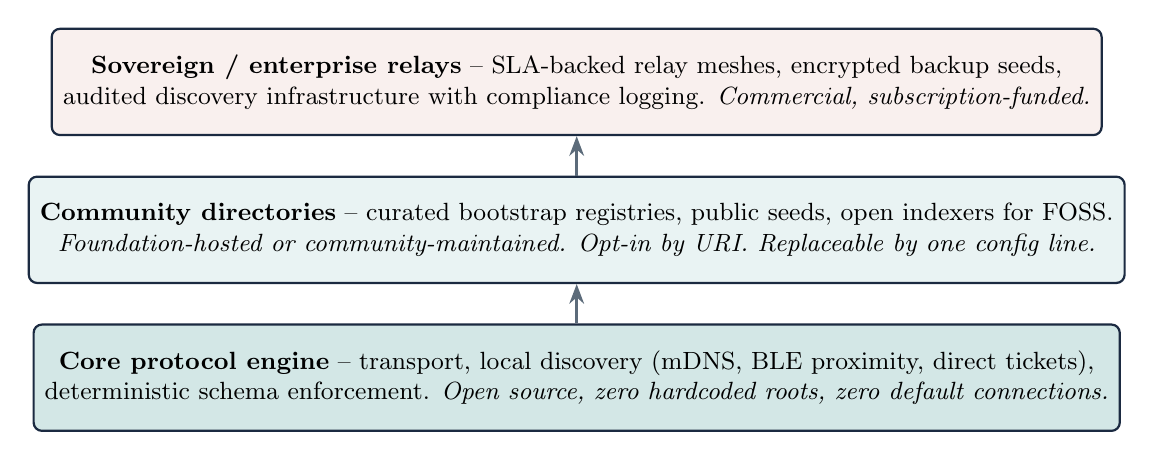
\begin{tikzpicture}[
  layer/.style={draw=ink, rounded corners=3pt, line width=0.8pt, minimum width=13.2cm,
                minimum height=1.35cm, align=center, font=\small, inner sep=4pt},
  arrow/.style={-{Stealth[length=2.5mm]}, line width=0.9pt, draw=mute}
]
  \node[layer, fill=accent!18] (core) {\textbf{Core protocol engine} -- transport, local discovery (mDNS, BLE proximity, direct tickets),\\deterministic schema enforcement. \emph{Open source, zero hardcoded roots, zero default connections.}};
  \node[layer, fill=accent!9, above=0.5cm of core] (dir) {\textbf{Community directories} -- curated bootstrap registries, public seeds, open indexers for FOSS.\\\emph{Foundation-hosted or community-maintained. Opt-in by URI. Replaceable by one config line.}};
  \node[layer, fill=warn!8, above=0.5cm of dir] (rel) {\textbf{Sovereign / enterprise relays} -- SLA-backed relay meshes, encrypted backup seeds,\\audited discovery infrastructure with compliance logging. \emph{Commercial, subscription-funded.}};
  \draw[arrow] (core.north) -- (dir.south);
  \draw[arrow] (dir.north) -- (rel.south);
\end{tikzpicture}
\caption{Decoupling the free protocol from the paid directory and relay services.}
\label{fig:layers}
\end{figure}

\begin{table}[H]
\centering\small
\begin{tabularx}{\textwidth}{@{}L{3.3cm}YY@{}}
\toprule
\textbf{Layer} & \textbf{Responsibility} & \textbf{Funding model} \\
\midrule
Core engine & P2P transport, local discovery, schema enforcement & Maintainer consortium; not dependent on any one sponsor \\
Community directories & Bootstrap registries, public seeds, indexers & Foundation or community; donations, memberships \\
Sovereign / enterprise relays & SLA-backed relays, backup seeds, compliance-logged discovery & Paid subscription; time-locked SLA streams; Slot~8 surety bonds \\
Hardware and deployment & Preconfigured nodes, packaging, support & Sales and service contracts; Slot~4 batch escrows \\
\bottomrule
\end{tabularx}
\caption{Who does what, and who pays.}
\end{table}

One concrete mechanism for the paid layers is specified in the Sovereign Bunny
whitebooklet: dynamic SLA escrows replace credit-card SaaS friction with time-locked
streams, and the SQLite Consortium and Ostrom's design principles supply the governance
precedent for funding a free core through the people who depend on it~\cite{ostrom1990,sqlite2025}.
A mid-size enterprise running a private mesh pays for an audited relay with compliance
logging, backed by operational surety bonds in Slot~8.

\subsection{Why disagreement is a feature}
\begin{itemize}
  \item \textbf{Forkability caps rent.} If a directory operator turns extractive, subscribers
        swap the directory in a single configuration line. The threat of exit disciplines
        the operator without any governance process.
  \item \textbf{Exit is rehearsed, not promised.} Export and restore
        should be a continuous CI drill (the whitebooklet specifies one for its ledger with bit-for-bit state-root equality).
        The same drill applies to a Radicle network: export manifest, refs and policy; restore elsewhere.
  \item \textbf{Blast radius is local.} A dispute inside one mesh never needs to be
        adjudicated by everyone.
\end{itemize}

% ============================================================================
\section{The technical remedy: networks as contexts, not places}
\label{sec:remedy}

\begin{figure}[H]
\centering
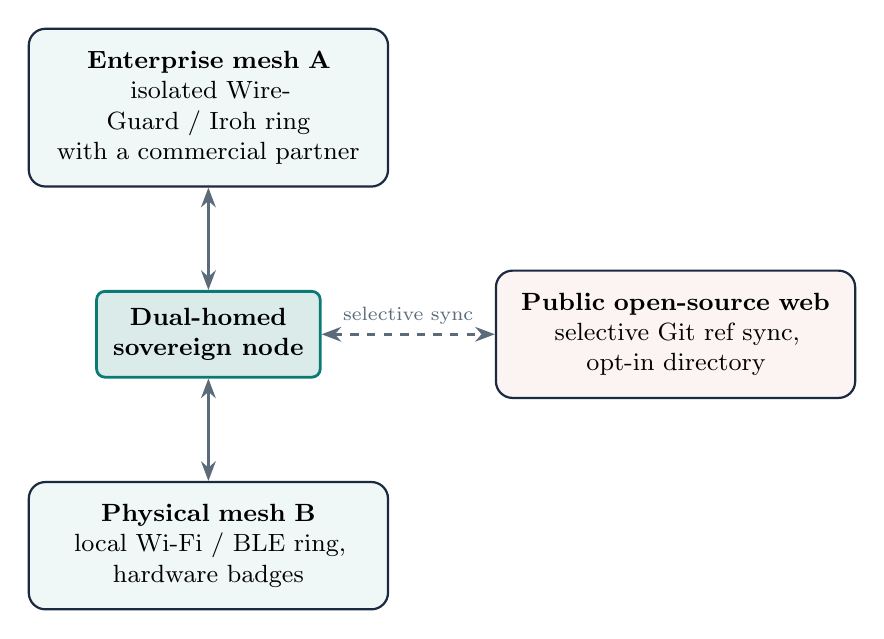
\begin{tikzpicture}[
  mesh/.style={draw=ink, rounded corners=6pt, line width=0.8pt, align=center, font=\small, inner sep=8pt, text width=4.0cm},
  nodebox/.style={draw=accent, fill=accent!15, rounded corners=3pt, line width=1pt, align=center, font=\small\bfseries, inner sep=6pt},
  link/.style={{Stealth[length=2.5mm]}-{Stealth[length=2.5mm]}, line width=0.9pt, draw=mute}
]
  \node[mesh, fill=accent!6] (a) {\textbf{Enterprise mesh A}\\isolated WireGuard / Iroh ring\\with a commercial partner};
  \node[nodebox, below=1.3cm of a] (n) {Dual-homed\\sovereign node};
  \node[mesh, fill=accent!6, below=1.3cm of n] (b) {\textbf{Physical mesh B}\\local Wi-Fi / BLE ring,\\hardware badges};
  \node[mesh, fill=warn!6, right=2.2cm of n] (p) {\textbf{Public open-source web}\\selective Git ref sync,\\opt-in directory};
  \draw[link] (a) -- (n);
  \draw[link] (n) -- (b);
  \draw[link, dashed] (n) -- node[above, font=\scriptsize, text=mute] {selective sync} (p);
\end{tikzpicture}
\caption{One node, three contexts. Each mesh need not know the others exist.}
\label{fig:dualhomed}
\end{figure}

A node may sit in a local Bluetooth or NFC mesh with physical badges, in an isolated ring
with an enterprise partner abroad, and selectively bridge public Git refs, without these three worlds
ever learning of one another. Three properties make this work.

\begin{enumerate}
  \item \textbf{Networks are contexts, not places.} Membership is a cryptographic fact, not an address.
  \item \textbf{Authorisation scopes discovery.} Capabilities determine what is routable. Peers
        discover only what they hold credentials to see.
  \item \textbf{No root of trust.} There is no canonical bootstrap list, no single gossip pool to
        pollute, and no ``the'' network to be banned from.
\end{enumerate}

\subsection{Scoped identifiers: \texttt{did:rad:<network\_id>:<subject>}}
\label{sec:scoped_did}

\begin{figure}[H]
\centering
\begin{lstlisting}[basicstyle=\ttfamily\small,frame=single,numbers=none,language={}]
did:rad:<network_id>:<peer_id_or_repo_id>
   |        |                  |
   |        |                  +-- Ed25519 public key / Git object hash
   |        +----------------------- BLAKE3 digest of the Genesis Trust Manifest
   +-------------------------------- method specification
\end{lstlisting}
\caption{Anatomy of a network-scoped identifier.}
\end{figure}

\paragraph{What defines \texttt{network\_id}?} Not an arbitrary label such as
\code{enterprise-internal}, but a digest of the \emph{Genesis Trust Manifest}: the
authorised relay keys, the default cryptographic suites, and the authorisation schema
(for us, a Zanzibar namespace configuration~\cite{pang2019zanzibar}). Two networks with
different rules therefore have different identifiers by construction.

\begin{lstlisting}[language=JSON,caption={Illustrative Genesis Trust Manifest (field names are a proposal, not a frozen format).}]
{
  "version": 1,
  "name_hint": "danish-pilot",
  "relay_keys": ["ed25519:<hex>", "ed25519:<hex>"],
  "crypto_suites": ["ed25519", "blake3"],
  "authz_schema": "blake3:<digest of zanzibar namespace config>",
  "directories": [],
  "bootstrap": []
}
\end{lstlisting}
Empty \code{directories} and \code{bootstrap} lists are valid and are the default:
the node starts without dialling anyone.

\paragraph{Cross-network identity.} The same hardware key may appear in several scopes,
and the scoped identifier differs per domain:
\begin{center}\small
\begin{tabular}{ll}
Public mesh: & \code{did:rad:public:z6Mkq\ldots}\\
Pilot network: & \code{did:rad:c7f8a9\ldots:z6Mkq\ldots}
\end{tabular}
\end{center}
Resolving a document under \code{did:rad:c7f8a9\ldots} evaluates the peer's permissions
strictly against \emph{that} network's state, which prevents cross-tenant privilege confusion.
Unlinkability between scopes is a design goal: a verifier in one network must not be able to
correlate scoped identifiers across networks without a deliberate disclosure by the holder
\claim{unverified: requires a per-scope key derivation, see \cref{sec:open}}.

\paragraph{Backward compatibility.} Existing \code{did:key} identities remain valid.
The current public mesh is simply \code{did:rad:public}; nothing existing is invalidated.

\subsection{The handshake firewall}
\label{sec:handshake}

The first authenticated frame of any connection carries the \code{network\_id}. If the identifiers
do not match, the connection is closed \emph{before} any routing table, inventory
announcement or repository reference is exchanged. Topological isolation then costs one
hash comparison.

\begin{lstlisting}[language=Rust,caption={Handshake gate (sketch). The comparison should be constant-time and must precede any application frame.}]
pub struct Hello {
    pub network_id: [u8; 32],   // BLAKE3(genesis trust manifest)
    pub peer_key:   [u8; 32],   // Ed25519, already authenticated by the transport
    pub nonce:      [u8; 16],
}

pub fn gate(local: &[u8; 32], hello: &Hello) -> Result<(), Reject> {
    // Constant-time compare; do not leak which byte differed.
    let mut diff = 0u8;
    for i in 0..32 {
        diff |= local[i] ^ hello.network_id[i];
    }
    if diff != 0 {
        return Err(Reject::NetworkMismatch); // close before any routing data
    }
    Ok(())
}
\end{lstlisting}

\begin{warnbox}{Honest limitation}
Sending \code{network\_id} in cleartext tells an observer which network you attempted to join.
Where that matters, the identifier should instead be proved inside the encrypted
transport session (for example as a pre-shared binding mixed into the handshake prologue),
or demonstrated by a keyed MAC, so a non-member learns nothing. We specify the
property, not yet the construction.
\end{warnbox}

\subsection{Capability-scoped discovery}
Inside a network, \emph{what} a peer learns is also scoped. Authorization is a relationship graph,
checked before announcement rather than after:
\begin{itemize}
  \item A node announces a repository identifier only to peers for which the tuple
        \code{repo:<rid>\#reader@peer:<did>} (or a rewrite reaching it) holds.
  \item Revoking the relationship stops future announcements; it cannot unsend what was already replicated,
        which is why scope is a discovery control and not a substitute for encryption at rest.
  \item The same tuple store drives roles, so there is no second access-control system to keep in sync.
\end{itemize}

\subsection{No hardcoded roots: the CLI contract}
\begin{lstlisting}[language={},basicstyle=\ttfamily\scriptsize,caption={Proposed operator workflow. The command names are illustrative.}]
# An isolated plant network: dials nothing
rad init --network-manifest ./manifest.json

# Join the wider public commons, explicitly and revocably
rad network subscribe did:rad:public --directory https://directory.example.org

# Walk away from a directory that went rogue
rad network unsubscribe --directory https://directory.example.org
\end{lstlisting}

% ============================================================================
\section{Names as a property of topology}
\label{sec:names}

Treating naming as a function of who connects to whom mirrors how physical networks actually work.

\subsection{Collision as a physical peering blocker}
In a flat mesh, routing needs unambiguous addresses. Two corporate networks that merge over a
tunnel with conflicting \code{192.168.1.0/24} subnets cannot route cleanly. The friction
is immediate and local: until it is resolved they cannot exchange invoices or push
commits. No court and no registry committee is required. The collision forces an economic choice: disambiguate,
bridge with a scoped prefix, or refuse to route.

\subsection{Concentric trust boundaries}
\begin{figure}[H]
\centering
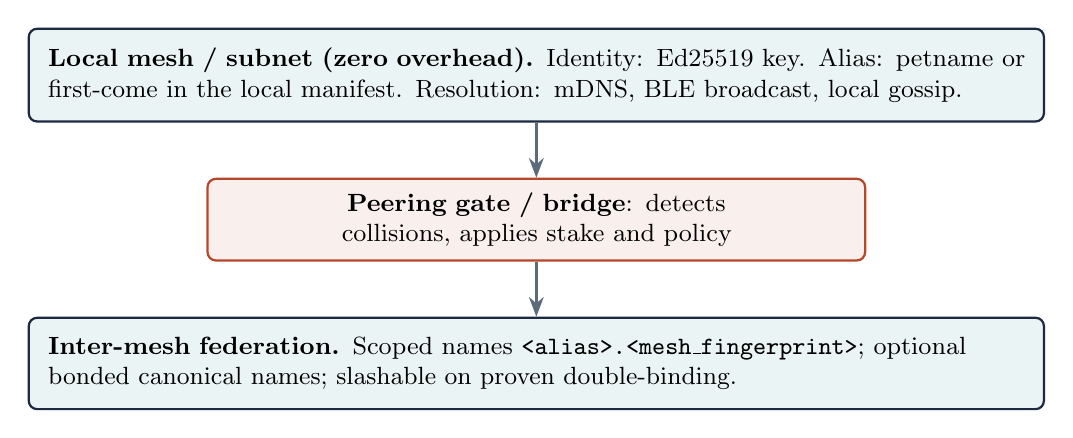
\begin{tikzpicture}[
  box/.style={draw=ink, rounded corners=3pt, line width=0.8pt, align=left, font=\small, inner sep=7pt, text width=12.4cm},
  gate/.style={draw=warn, fill=warn!8, rounded corners=3pt, line width=0.8pt, align=center, font=\small, inner sep=5pt, text width=8cm},
  arrow/.style={-{Stealth[length=2.5mm]}, line width=0.9pt, draw=mute}
]
  \node[box, fill=accent!8] (local) {\textbf{Local mesh / subnet (zero overhead).} Identity: Ed25519 key. Alias: petname or first-come in the local manifest. Resolution: mDNS, BLE broadcast, local gossip.};
  \node[gate, below=0.7cm of local] (g) {\textbf{Peering gate / bridge}: detects collisions, applies stake and policy};
  \node[box, fill=accent!8, below=0.7cm of g] (fed) {\textbf{Inter-mesh federation.} Scoped names \code{<alias>.<mesh\_fingerprint>}; optional bonded canonical names; slashable on proven double-binding.};
  \draw[arrow] (local) -- (g);
  \draw[arrow] (g) -- (fed);
\end{tikzpicture}
\caption{Names are claims bound to keys, scoped by default.}
\end{figure}

\begin{itemize}
  \item \textbf{Cryptographic origin.} Every entity is a key. Human-readable names are never
        absolute; they are claims mapped to keys.
  \item \textbf{Scoped prefix as default.} If two networks both claim \code{auth-gateway}, a federating
        resolver renders them \code{auth-gateway.funkfeuer-vie} and \code{auth-gateway.cbase-ber}.
        Dropping the qualifier to claim a canonical root is an economic act, not a technical default.
  \item \textbf{Bonded, non-equivocating routing slots (optional).} A peer that wants a canonical
        route in a shared community mesh posts a bond. Two contradictory signed bindings for the same
        name are a self-contained proof that burns the bond. This requires a ledger for bonds
        and is therefore an \emph{optional} layer for networks that choose to attach one (a stateless account-lattice as in the whitebooklet is one such choice); the core does not need it.
  \item \textbf{Directories as convenience.} A community index of reputable names is a subscription
        feed, replaceable at any time, or bypassed by direct peer discovery.
\end{itemize}

% ============================================================================
\section{Graph of graphs: macro-nodes, boundaries and intents}
\label{sec:graphs}

\subsection{Local density, macro abstraction}
Inside a cluster (an ERP deployment, a wireless mesh, a team) nodes have high relational density
and low-latency trust, talk over local transports, and do not care about the wider internet. To the
outside the whole cluster condenses into one macro-node with an aggregate capacity, an
attestation record and a bonded commitment. This is how the physical Internet already scales:
BGP routes between autonomous systems on peering agreements, not between individual laptops.

\subsection{The boundary as an economic checkpoint}
At the boundary the rules invert. Inside cluster A, node 1 trusts gateway A. Cluster B has no
reason to accept an unverified claim from an unknown foreign node, and it need not: transit is cleared
by the \emph{cluster's} reputation and stake, not by individual identity. A rogue node inside A can be rejected
locally; its misbehaviour never reaches the wider graph unless gateway A is willing to forward it
with its own macro-reputation on the line.

\subsection{Intent-based routing}
\emph{Status: \stRes{}.} From the initiator's point of view the transport rails are an implementation
detail. The originator emits a signed intent (``reconcile this claim against release v2.4.1, settle the
amount to this destination, maximum fee budget $x$''). Independent solvers and boundary relays find a path across
their local quotient graphs; each intermediate macro-network takes a fractional fee for fronting counterparty
risk and checking the boundary invariant. The sender does not care whose infrastructure carries the payload, only
that a cryptographic path exists, the hops preserve non-repudiation, and settlement balances. A clearing layer is assumed; the whitebooklet's multilateral netting is one candidate, not a requirement.

% ============================================================================
\section{Risks of giving up control}
\label{sec:risks}

Polycentricity is not free. We list the failure modes we expect and the mitigation we propose.

\begin{table}[H]
\centering\small
\begin{tabularx}{\textwidth}{@{}L{3.1cm}YY@{}}
\toprule
\textbf{Risk} & \textbf{How it shows up} & \textbf{Mitigation} \\
\midrule
Fragmentation & Many small networks, weak discovery between them & Opt-in directories, bridges, intent routing; accept some loss as the price of sovereignty \\
Eclipse / isolation & A node's only peers are adversarial & Multiple independent directories; multi-seed diversity threshold $m_{\min}$ \\
Name-collision spam & Cheap claims flood a shared mesh & Scoped prefixes by default; stake for canonical names \\
Directory capture & A directory operator censors or skews & Replaceable by one line; observer-relative ranking of directories \\
Fork confusion & Users cannot tell the real network & \code{network\_id} is a digest of rules, so lookalikes differ verifiably \\
Cleartext network label & Observers learn which network a node joins & Prove the binding inside the encrypted session (\cref{sec:handshake}) \\
Cross-scope correlation & Same key links identities across networks & Per-scope key derivation (open problem, \cref{sec:open}) \\
\bottomrule
\end{tabularx}
\caption{Risk register for a polycentric network.}
\end{table}

% ============================================================================
\section{Roadmap}
\label{sec:roadmap}
\begin{enumerate}
  \item \textbf{Phase 0 -- Document and verify.} Re-check every claim marked reported in \cref{sec:verify} against the current upstream tree, and run the seed-concentration crawl. Open a design discussion rather than a pull request.
  \item \textbf{Phase 1 -- Configuration only.} Ship a documented ``isolated network'' profile (no default seeds, explicit directory subscription) with no protocol change.
  \item \textbf{Phase 2 -- \texttt{network\_id} gate.} Add the network identifier to the handshake, defaulting to \code{public} for backward compatibility.
  \item \textbf{Phase 3 -- Scoped DIDs and tuple-gated announcements.}
  \item \textbf{Phase 4 -- Directories and relays as products.} Publish the directory protocol, run a reference community directory, and offer SLA-backed relays.
  \item \textbf{Phase 5 -- Bonded names and intents (optional, research).}
\end{enumerate}

\section{Open problems}
\label{sec:open}
\begin{itemize}
  \item A handshake construction in which a non-member learns nothing about the network identifier.
  \item Per-scope key derivation that preserves hardware-badge usability while keeping scopes unlinkable.
  \item Directory ranking that resists Sybil flooding without a central curator.
  \item A migration path that lets existing repository identifiers be re-expressed under scoped identifiers without breaking links.
  \item Economic parameters (bond sizes, relay fee splits) are \claim{unverified} hypotheses and require simulation before any deployment.
\end{itemize}

\section{Status of upstream claims}
\label{sec:verify}
Checked on 2026-10-17 against primary sources reachable from the authoring environment: the project's FAQ, its security-disclosure announcement as linked from the FAQ and summarised by public reports, the Radicle Garden service page, and the arXiv record of the Lightning study. Source-code claims were supplied by a reviewer reading the upstream tree; we have not re-read the code, so they are marked \claim{reported}, and any of them that turns out wrong must be corrected here before public circulation.

\begin{table}[H]
\centering\small
\begin{tabularx}{\textwidth}{@{}L{0.8cm}YL{2.5cm}@{}}
\toprule
\textbf{ID} & \textbf{Claim} & \textbf{Status} \\
\midrule
V1 & Default bootstrap nodes on the main network, hosted by the foundation; an empty list on the test network; no dedicated switch for an isolated network (manual configuration and peer-database reset) & reported \\
V2 & The only network-level configuration is a two-value main/test selector choosing directories and bootstrap defaults; no network identifier is verified in the handshake & reported \\
V3 & Three signed announcement types (node, inventory, refs); inventory announcements reveal seeded public repositories to the pool; private repositories use a flat allow-list of keys and are omitted from inventory & reported \\
V4 & \code{rad seed} (repository level, with a scope option) and \code{rad follow} (peer level) replaced \code{rad track} & reported (FAQ confirms seed policies; verb split not re-checked) \\
V5 & Peer identity is \code{did:key} only; repository identifiers are hash-derived; no network-scoped DID method or external resolver & reported \\
V6 & Grants from Radworks, maintainer-led, no blockchain dependence (FAQ); hosted seed service at 4.99 euro per month run by the foundation (service page); size of 2026 grants and profit recycling & verified (first two); reported (grant amount, profit recycling) \\
V7 & Seed concentration: the FAQ figures (about 8{,}000 repositories, 600+ nodes weekly) are a lower bound seen by the foundation's own seeds and explicitly a proper subset of activity; they do not measure how much is reachable only via a few operators & \textbf{not supported as evidence}; needs a real measurement \\
V8 & Lightning hub concentration: Lin et al.\ (Gini of node strengths about 0.88; 10\% of nodes hold about 80\% of funds; hub removal fragments the graph), data 2018--2019 & verified (cited study); post-2019 persistence unverified \\
V9 & Affected releases of the disclosed flaw (reported as up to 1.10.3) and the exact Iroh migration plan and timing & reported; migration completion unverified \\
\bottomrule
\end{tabularx}
\caption{Verification status. ``Verified'' means checked against a primary source by us; ``reported'' means supplied but not independently re-checked.}
\end{table}

\paragraph{A correction to a tempting inference.} The FAQ's repository and node counts have been offered as direct confirmation of seed-node gravity. They are not: the FAQ warns that the figures are likely a proper subset of network activity, and a count of what one operator's seeds observe says nothing about the fraction of repositories reachable through them alone. The gravity thesis rests instead on (i) the FAQ's statement that NAT-bound peers currently depend on seed nodes, (ii) reported default bootstrap configuration, and (iii) the Lightning precedent as an analogy. A decisive test would crawl the public network and compute, per repository, the number of independent seed operators that announce it.

\section{Conclusion}
Radicle already did the harder half: it removed code collaboration from a monolithic
global state machine. The remaining half is to stop treating the network as a single room. Scope identity and discovery to
a cryptographically named network; make every directory and seed a replaceable choice; and fund the work by selling
services around a free core that anyone may run, including those who disagree with us. That shifts the posture from an
imperial model in which everyone connects to the mother ship by default, to an emergent web of sovereign meshes that peer
only when it serves a purpose, and it gives the maintainers permission to stop being martyrs.

\begin{thebibliography}{9}
\bibitem{radicle2024} Radicle Foundation. \emph{Radicle: A Sovereign Peer-to-Peer Protocol for Code Collaboration}. 2024. \url{https://radicle.xyz/}
\bibitem{pang2019zanzibar} R.~Pang et al. Zanzibar: Google's Consistent, Global Authorization System. \emph{USENIX ATC}, 2019, pp.~923--935.
\bibitem{ostrom1990} E.~Ostrom. \emph{Governing the Commons: The Evolution of Institutions for Collective Action}. Cambridge University Press, 1990.
\bibitem{sqlite2025} SQLite Consortium. \emph{SQLite Consortium}. \url{https://sqlite.org/consortium.html}
\bibitem{lin2020lightning} J.-H.~Lin, K.~Primicerio, T.~Squartini, C.~Decker, C.~J.~Tessone. Lightning Network: a second path towards centralisation of the Bitcoin economy. \emph{New Journal of Physics} 22, 083022, 2020. arXiv:2002.02819.
\bibitem{radiclefaq} Radicle project. \emph{Frequently asked questions}. \url{https://radicle.dev/faq} (accessed 2026-10-17).
\bibitem{radicledisclosure} Radicle project. \emph{Disclosure of vulnerability in network protocol}, 2026-09-23 (linked from the FAQ). \url{https://radicle.dev/2026/09/23/disclosure-of-vulnerability-in-network-protocol.html}
\bibitem{radiclegarden} Better Internet Foundation. \emph{Radicle Garden}. \url{https://radicle.garden/} (accessed 2026-10-17).
\bibitem{mica2023} European Parliament and Council of the European Union. \emph{Regulation (EU) 2023/1114 on markets in crypto-assets (MiCA)}. Official Journal of the European Union, L 150, 9 June 2023, pp.~40--149.
\end{thebibliography}

\end{document}
